%%% The main file. It contains definitions of basic parameters and includes all other parts.

%% Settings for single-side (simplex) printing
% Margins: left 40mm, right 25mm, top and bottom 25mm
% (but beware, LaTeX adds 1in implicitly)
\documentclass[12pt,a4paper]{report}
\setlength\textwidth{145mm}
\setlength\textheight{247mm}
\setlength\oddsidemargin{15mm}
\setlength\evensidemargin{15mm}
\setlength\topmargin{0mm}
\setlength\headsep{0mm}
\setlength\headheight{0mm}
% \openright makes the following text appear on a right-hand page
\let\openright=\clearpage


%% Settings for two-sided (duplex) printing
% \documentclass[12pt,a4paper,twoside,openright]{report}
% \setlength\textwidth{145mm}
% \setlength\textheight{247mm}
% \setlength\oddsidemargin{14.2mm}
% \setlength\evensidemargin{0mm}
% \setlength\topmargin{0mm}
% \setlength\headsep{0mm}
% \setlength\headheight{0mm}
% \let\openright=\cleardoublepage

%% Generate PDF/A-2u
\usepackage[a-2u]{pdfx}

%% Character encoding: usually latin2, cp1250 or utf8:
\usepackage[utf8]{inputenc}

%% Prefer Latin Modern fonts
\usepackage{lmodern}

%% Further useful packages (included in most LaTeX distributions)
\usepackage{amsmath}        % extensions for typesetting of math
\usepackage{amsfonts}       % math fonts
\usepackage{amsthm}         % theorems, definitions, etc.
\usepackage{bbding}         % various symbols (squares, asterisks, scissors, ...)
\usepackage{bm}             % boldface symbols (\bm)
\usepackage{graphicx}       % embedding of pictures
\usepackage{fancyvrb}       % improved verbatim environment
\usepackage{natbib}         % citation style AUTHOR (YEAR), or AUTHOR [NUMBER]
\usepackage[nottoc]{tocbibind} % makes sure that bibliography and the lists
			    % of figures/tables are included in the table
			    % of contents
\usepackage{dcolumn}        % improved alignment of table columns
\usepackage{booktabs}       % improved horizontal lines in tables
\usepackage{paralist}       % improved enumerate and itemize
\usepackage{xcolor}         % typesetting in color
\usepackage{subcaption}
\usepackage[ruled]{algorithm2e}
\usepackage[acronym,toc,shortcuts,nonumberlist]{glossaries}
\usepackage{diagbox}


\usepackage{color}
\definecolor{bluekeywords}{rgb}{0.13,0.13,1}
\definecolor{greencomments}{rgb}{0,0.5,0}
\definecolor{redstrings}{rgb}{0.9,0,0}

\usepackage{listings}
\lstset{language=[Sharp]C,
  showspaces=false,
  showtabs=false,
  breaklines=true,
  showstringspaces=false,
  breakatwhitespace=true,
  escapeinside={(*@}{@*)},
  commentstyle=\color{greencomments},
  keywordstyle=\color{bluekeywords},
  stringstyle=\color{redstrings},
  basicstyle=\ttfamily
}

\newacronym{AI}{AI}{Artificial Intelligence}
\newacronym{XR}{XR}{extended reality}
\newacronym{RTS}{RTS}{real-time strategy}
\newacronym{MCTS}{MCTS}{Monte-Carlo tree search}
\newacronym{Csharp}{C\#}{C Sharp}
\newacronym{OOP}{OOP}{Object Oriented Programming}

\makeglossaries


%%% Basic information on the thesis

% Thesis title in English (exactly as in the formal assignment)
\def\ThesisTitle{Artificial Intelligence for Quoridor game}

% Author of the thesis
\def\ThesisAuthor{Devyanshu Koirala}

% Year when the thesis is submitted
\def\YearSubmitted{2024}

% Name of the department or institute, where the work was officially assigned
% (according to the Organizational Structure of MFF UK in English,
% or a full name of a department outside MFF)
\def\Department{Department of Software and Computer Science Education (KSVI)}

% Is it a department (katedra), or an institute (ústav)?
\def\DeptType{Department}

% Thesis supervisor: name, surname and titles
\def\Supervisor{Mgr. Klára Pešková, Ph.D.}

% Supervisor's department (again according to Organizational structure of MFF)
\def\SupervisorsDepartment{KSVI}

% Study programme and specialization
\def\StudyProgramme{Computer Science}
\def\StudyBranch{Artificial Intelligence (AI)}

% An optional dedication: you can thank whomever you wish (your supervisor,
% consultant, a person who lent the software, etc.)
\def\Dedication{%
I would like to express my deepest gratitude to my supervisor, Mgr. Klára Pešková, Ph.D for her invaluable guidance and support. Her mentorship, expertise, dedication and constructive feedbacks have been vital throughout this journey.

Furthermore the constant support and encouragement from my friends and family have been my guiding light. To my family for always believing in my potential and for motivating me throughout my academic journey, my friends and my brother, who have played countless games of Quoridor with me in order to help me understand the game on a deeper level, I will forever be grateful.
}

% Abstract (recommended length around 80-200 words; this is not a copy of your thesis assignment!)
\def\Abstract{%
Quoridor presents a challenging terrain for strategic decision-making, making it a suitable testing ground for various Artificial Intelligence (AI) algorithms. This thesis explores the implementation of generic interfaces for AI agents and finally evaluation the AI agents in the game, namely Minimax, Monte Carlo Tree Search (MCTS) and A-star within the realm of Quoridor gameplay. In the thesis, we develop the AI interface that can be easily integrated into any other game. 

The research begins with a comprehensive overview of the Quoridor game, its rules and strategies. Subsequently, we delve into the theoretical foundations and practical implementation details of the aforementioned AI algorithms and conduct a thorough evaluation in an effort to determine the best one in this context.
}

% 3 to 5 keywords (recommended), each enclosed in curly braces
\def\Keywords{%
{Quoridor} {Artificial Intelligence} {AI} {Board Game}
}

%% The hyperref package for clickable links in PDF and also for storing
%% metadata to PDF (including the table of contents).
%% Most settings are pre-set by the pdfx package.
\hypersetup{unicode}
\hypersetup{breaklinks=true}

% Definitions of macros (see description inside)


% Title page and various mandatory informational pages
\begin{document}
%%% Title page of the thesis and other mandatory pages

%%% Title page of the thesis

\pagestyle{empty}
\hypersetup{pageanchor=false}
\begin{center}

\centerline{\mbox{
\includegraphics[width=166mm]{../img/logo-en.pdf}}}

\vspace{-8mm}
\vfill

{\bf\Large BACHELOR THESIS}

\vfill

{\LARGE\ThesisAuthor}

\vspace{15mm}

{\LARGE\bfseries\ThesisTitle}

\vfill

\Department

\vfill

{
\centerline{\vbox{\halign{\hbox to 0.45\hsize{\hfil #}&\hskip 0.5em\parbox[t]{0.45\hsize}{\raggedright #}\cr
Supervisor of the bachelor thesis:&\Supervisor \cr
\noalign{\vspace{2mm}}
Study programme:&\StudyProgramme \cr
\noalign{\vspace{2mm}}
Study branch:&\StudyBranch \cr
}}}}

\vfill

% Zde doplňte rok
Prague \YearSubmitted

\end{center}

\newpage

%%% Here should be a bound sheet included -- a signed copy of the "bachelor
%%% thesis assignment". This assignment is NOT a part of the electronic
%%% version of the thesis. DO NOT SCAN.

%%% A page with a solemn declaration to the bachelor thesis

\openright
\hypersetup{pageanchor=true}
\pagestyle{plain}
\pagenumbering{roman}
\vglue 0pt plus 1fill

\noindent
I declare that I carried out this bachelor thesis independently, and only with the cited
sources, literature and other professional sources. It has not been used to obtain another
or the same degree.

\medskip\noindent
I understand that my work relates to the rights and obligations under the Act No.~121/2000 Sb.,
the Copyright Act, as amended, in particular the fact that the Charles
University has the right to conclude a license agreement on the use of this
work as a school work pursuant to Section 60 subsection 1 of the Copyright~Act.

\vspace{10mm}

\hbox{\hbox to 0.5\hsize{%
In \hbox to 6em{\dotfill} date \hbox to 6em{\dotfill}
\hss}\hbox to 0.5\hsize{\dotfill\quad}}
\smallskip
\hbox{\hbox to 0.5\hsize{}\hbox to 0.5\hsize{\hfil Author's signature\hfil}}

\vspace{20mm}
\newpage

%%% Dedication

\openright

\noindent
\Dedication

\newpage

%%% Mandatory information page of the thesis

\openright

\vbox to 0.5\vsize{
\setlength\parindent{0mm}
\setlength\parskip{5mm}

Title:
\ThesisTitle

Author:
\ThesisAuthor

\DeptType:
\Department

Supervisor:
\Supervisor, \SupervisorsDepartment

Abstract:
\Abstract

Keywords:
\Keywords

\vss}

\newpage

\openright
\pagestyle{plain}
\pagenumbering{arabic}
\setcounter{page}{1}


%%% A page with automatically generated table of contents of the bachelor thesis

\tableofcontents

%%% Each chapter is kept in a separate file
\chapter{Introduction}
\addcontentsline{toc}{chapter}{Introduction}

\section{Overview}
In recent years, \ac{AI} is becoming an integral part of many elements of modern world including gaming \citep{Skinner2010Artificial}, pushing the boundaries of what's achievable in both single and multiplayer gaming experiences. \ac{AI}-driven games now offer users the opportunity to hone and enhance their skills, providing varying difficulty levels and offering optimal moves to guide players through each step if desired. \ac{AI} has also taken a center stage in gaming with its remarkable accomplishments in age-old strategy games such as Chess, Go, and many others. 

% . In fact, in the recent years, it has become an the main point of evolution and revolution in many of the technologies and industries. From assisted or autonomous driving \citep{Ma2020Artificial}, chat bots \citep{Wu2023ABrief} to gaming \citep{Skinner2010Artificial}, it has been a major revelation in evolving the existing technologies to generating new industry space with the plethora of new use cases.   
% 

Strategy games are a genre of gaming that require planning, often involving various tactics, decision making and execution under various resource constraints. Some examples of strategy games include Chess, Go, Shogi and Starcraft. They are unique compared to other genres as they require a selection of an optimal move among multiple possible moves based certain strategy. In many scenarios, the size of possible moves depends on the game tree, simulation and prediction of the player's and the opponent's moves all while managing resources efficiently.

\ac{AI}, due to its suitability of solving complex decision making problems factoring in multiple variable and constraints, has been particularly effective in playing the strategy games. The history of \ac{AI} in strategy gaming dates few decades. One of the initial marked impact of \ac{AI} in the strategy gaming came in 1997 when IBM's Deep Blue \citep{Campbell2002Deep} defeated World Chess Champion Garry Kasparov. The influence was more prominent with the success of \ac{AI} on \ac{RTS} games such as Warcraft and StarCraft \citep{Robertson2014Review} and strategy games such as Go \citep{Huang2011Monte}. Recently, DeepMind's Alpha Go for Go, Alpha Zero for Chess \citep{Silver2017Mastering} and AlphaStar for StarCraft \citep{Team2019Alphastar} have widened the gap between the \ac{AI} and human intelligence even further.


\section{Quoridor}

Designed by Mirko Marchesi, Quoridor stands out as an engaging strategic board game that is played between two or four players. The game is played on a square grid board where the objective of this game is for each player to move their pawn to the opposite side of the board. This game introduces a fascinating twist where a player, in addition to trying to move their pawn through the square grid, additionally have an option to place walls on the grid locations strategically to obstruct the opponent's path. This strategy compels the player to think of their traversal strategy while predicting the opponents strategy as well. Despite its seemingly simple rules, Quoridor demands a unique blend of strategic foresight and the ability to anticipate the moves of opponents and outmaneuver the opponent.


\section{AI algorithms overview}
In this section, we give a brief overview of different \ac{AI} techniques that have been considered in this thesis.

\subsection{Minimax algorithm}
Minimax algorithm, first proven by John von Neumann in 1928 in his paper \textit{Zur Theorie Der Gesellschaftsspiele} \citep{v1928theorie}, is a very popular algorithm employed in many decision-making scenarios for e.g., in decision theory, game theory and even philosophy. As suggested by the name minimax, the idea of the algorithm is to minimize the player's loss when the opponent makes a decision that gives the player the maximum loss. This algorithm has been implemented in many multi-player strategy games such as tic-tac-toe \citep{savelli2008tic}. 

The minimax algorithm involves in the player performing an exhaustive search on the game tree to determine a sequence of maximizing and minimizing moves. The complexity of such algorithm in large game tree often means such search is often impossible due to limited computational resources. To limit this complexity, further techniques such as depth-limited minimax, alpha-beta pruning and parallel minimax algorithm can be used.

\subsection{Monte-Carlo Tree Search}
\ac{MCTS} \citep{Coulom2006Efficient} is a heuristic tree search algorithm popular in decision-making processes, mostly popular in strategic games where the game tree space is too large to traverse. One problem with the minimax algorithm is that it requires a robust and accurate evaluation function to evaluate a given position in the game. This problem can be even more relevant when the game tree space is too large making it difficult to find the evaluation of a position. The basic idea of the \ac{MCTS} algorithm is that is narrows down on certain areas of the game tree, such that the exhaustive traversal and search of the tree is not required. The algorithm achieves this by taking random samples in the tree space and building a search tree based on it.

\subsection{A-star algorithm}
A star is a popular algorithm \citep{Hart1968AFormal} used mainly for graph search and traversal problems. The main aim of the A-star algorithm is to find a path between a starting node and an destination node with the least cost. The algorithm 


\section {Acknowledged Works}

Compared to some other strategy games such as Chess and Go, Quoridor has not been extensively studied in the literature. In \citep{Glendenning2002MasteringQ}, the author developed an agent for playing Quoridor using genetic algorithm to optimize the weights. The authors in \citep{Mertens2006Quoridor} study the complexity of the algorithm also develop a Quoridor playing agent based on Minimax algorithm. Likewise, the authors in \citep{Brenner2015Artificial} developed an \ac{MCTS} approach for Quoridor. Recently, in \citep{Iwanaga2022Analysis}, the authors performed an analysis of the game for a miniature 5 by 5 board.


Quoridor, being a widely popular game, has attracted a fair number of attention from the research community,
resulting in successful AI agent developments. Some of the notable works include:

\begin{itemize}
    \item \textbf{Mastering Quoridor \citep{Glendenning2002MasteringQ}}
    The writer implements and assesses various algorithms like Negamax, Alpha-beta negamax among others.
    Additionally, they utilized a genetic algorithm to refine the weights within a linear weighted evaluation
    function, employing 10 distinct features suggested by the author, some of which include player's position
    towards their goal side, the opponent's position towards their respective goal, the remaining count of
    walls available to the player, etc.
\end{itemize}


In sharp contrast to the aforementioned paper, our thesis takes a distinctly different path by delving deeply
into the architectural aspects of AI. Our approach emphasizes abstraction to the greatest extent possible, with
an eye on facilitating seamless integration into a broad spectrum of games. We prioritize creating an
interface that is adaptable to diverse game environments, setting our research apart from the game-specific
focus of the prior works.






The primary objective of this thesis is to construct a well-structured framework and user-friendly interfaces
that seamlessly integrate AI algorithms into the Quoridor game. The development of AI algorithms customized to
Quoridor's unique rule set will not only enhance our understanding of the game's intricate nuances but also
facilitate the creation of an intuitive interface for simulating these AI agents. Furthermore, a comprehensive
evaluation will be conducted to identify the top-performing AI agent.

In addition to this, the project will encompass the creation of a user-friendly interface that empowers players
to engage with an AI opponent of their choice, thereby bolstering the game's accessibility and inclusivity.




\chapter{Quoridor: Game description}
\label{GameDescription}

Quoridor is a 2, or 4 player game played in an NxN chess-like board where each player has a pawn and a set number of walls, where, typically the dimension of N is an odd number with 9x9 board being the most popular. In the game, each square represents a potential position for the pawn pieces. The board also contains grooves bordering each squares on the board where the player can place the walls. With 9x9 board, the total number of walls available to the player is 10.

The game starts with the pawn pieces of the players on the opposite side of the NxN square board. The starting position of the pawn is the center of the edge of the board associated with the side of the player. Each player, additionally, can place a wall on the grooves of the board between any two squares. The main objective is to be the first player to traverse with the pawn through the board to any one of the N squares on the opposite edge of the board. A player, in their each move, can either move a pawn or place a wall. The idea is that placing the wall between the squares means that the opponent cannot pass through the squares and potentially many need to take a longer route to reach the opposite edge of the board. Hence, the strategy of a player in the game is to be the first player to move
their pawn to the row of squares on the opposite edge of the game board avoiding any walls deterring its path to the goal while strategically placing walls to deter opponents from reaching their goal squares.

The Quoridor game is played in turns between the opponents where in each turn the player can either move a pawn or place a wall. Then the move shifts to the opponent player(s) where they can do the same in their turn.

Walls are a fundamental element of the game, allowing players to strategically block their opponent's path and influence the course of the game. Each wall spans across two squares on the board and occupies exactly four squares either horizontally or vertically, effectively creating a barrier between them. At the beginning, each player starts
with a set number of walls that they can use during their turn.

\begin{figure}[!ht]
    \centering
    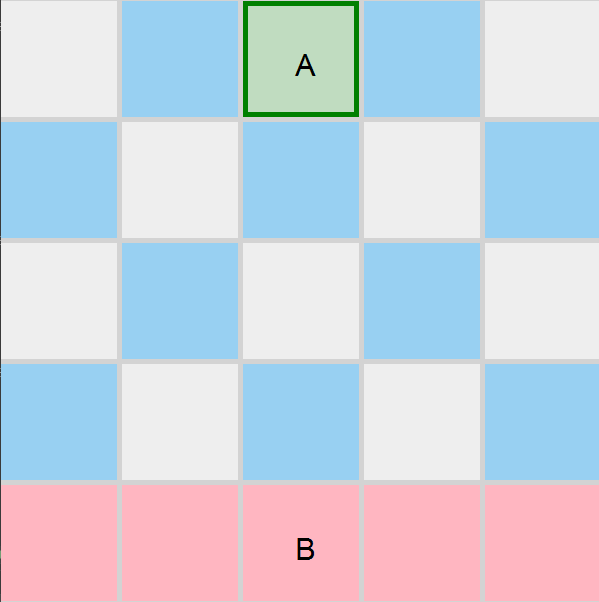
\includegraphics[scale=0.25]{../img/GameBoard/initial.png}
    \caption{A screenshot of a 5x5 game board from our implementation}
    \label{fig:InitialGameBoard}
\end{figure}

As seen in Figure \ref{fig:InitialGameBoard}, in this thesis, we consider a two-player Quoridor game with player A and player B. The pawn of player A is represented by the letter 'A' and that of player B is represented by the letter 'B'. In the figure, we display a 5x5 board with the squares on the edge of the board highlighted in pink belonging to player B whereas the squares on the opposite edge of the board belonging to player A. The board in the figure also shows the starting position of the two players with the pawn at the center of their respective edges. The goal of player A is to move its pawn through the board to one of the squares on the edge belonging to player B that has been highlighted in pink. The gray areas between the squares on the board represents the grooves of the board where walls can be placed. As mentioned earlier, the length of the walls is equal to the length of two squares. Hence, placing a wall on the board touches four squares where two squares are on one side of the wall whereas the two other squares are on the opposite side of the wall. The player cannot cross the squares through the wall. 

In order to formalize the game, we have to define the notations and use it to formally define the game rules and the player movement and wall placement rules.

\section{Notation}

In this subsection, we will first consider the notations popular in the literature and the Quoridor community and then define our own notation, especially for the wall placement, while analyzing the differences between them. This definition of our own notation is motivation by the ambiguity that we present existing in the current notation.

There are no official notations for this game. However, some popular ones recognized by the Quoridor community
include \textbf{Glendenning's Notation} (\citep{Glendenning2002MasteringQ}) and the \textbf{Quoridor Strat's Notation}
(\citep{website:COMMUNITY_NOTATION}). We first consider the notations in these two references below:

First, defining the notation of the squares of the board, consider a Quoridor board of dimension 9x9 as an example. Let $\mathbb{K} = \{a, ..., i\}$ and $\mathbb{R} = \{1, ..., 9\}$ and $C$ denote the 2D Quoridor board with $C_{i,j}$ representing the $i$-th row and $j$-th column position of the cell. Both the Glendenning's and Quoridor Strat's notations follow the same principle of labelling each cell or a square by $C_{i,j}$ where $i \in \mathbb{R}$ and $j \in \mathbb{K}$. Hence, in this approach the board is labelled by a combination of alphabetical letters (e.g., $\mathbb{K}$) denoting the columns and the positive integers (e.g., $\mathbb{R}$) representing the rows. This follows the similar style of notation for labelling the squares in chess.

This notation can be extended to a Quoridor board of any dimension NxN by considering the dimension of both $\mathbb{K}$ and $\mathbb{R}$ as $N$ where $\mathbb{K}$ is the set of first $N$ alphabetical characters in an ascending order and $\mathbb{R}$ is the set of first $N$ positive integers in a ascending order.


Considering an example in Figure \ref{fig:InitialGameBoard}, with these notations, the pawn A is in the position $C_{1, c}$ and the pawn B is in the position $C_{5, c}$.

After representing the Quoridor board, the next step for defining notations for the game is to define the moves. Let us represent the move for a player as $M$.

\begin{equation}\label{eqn:movement}
M(C_{ij}) = ji \text{, where, } j \in \mathbb{K} \text{ and, } i \in \mathbb{R}     
\end{equation}

Unlike in chess, in Quoridor, there is only one pawn for each side. Hence, for the side, for moving the pawn, the starting position of the pawn is not required. Hence, as mention in Equation \eqref{eqn:movement}, the movement of the pawn to the cell $C_{j, i}$ can simply be defined by the notation $ji$. The movement of the pawn A, in Figure \ref{fig:InitialGameBoard} from its position from cell $C_{1, c}$ to the position of B in $C_{5,c}$ through the cells $C_{2, c}$, $C_{3, c}$ and $C_{4, c}$ can be defined with moves $c2$, $c3$, $c4$ and $c4$ requiring a total of 4 moves.

Additionally, as described earlier, the Quoridor game is played between multiple players where each player in a turn can make a move. Hence, the turns are represented numerically, for e.g., 1., 2., 3. represents the first, second and third move respectively. Hence considering the scenario where player A moves its pawn in Figure \ref{fig:InitialGameBoard} from $C_{1,c}$ to $C_{2,c}$ and then to $C_{3,c}$ and player B moves its pawn from $C_{5,c}$ to $C_{4,c}$ to $C_{4,b}$, the notations can be represented as: $1. C2 C4$, $2. C3 B4$. Here the numbers 1. and 2. represents the two moves of each players and $1. C2 c4$ represents the movement of the players A's pawn to C2 and then player B's pawn to C4. The order of the player's movement can be dependent on the player that moves first. For example, in the example, player A moves first to $C4$, hence it is notated before player B's move. This order has to remain constant throughout the game.

Similarly, after notation of the board and the movement, the notation for wall placement is another important component for Quoridor. The notation for wall placement is defined by the following equations:

\begin{equation}\label{eqn:wall1}
W(C_{i,j}) = jiD \text{ , where, } j \in \mathbb{K}, i \in \mathbb{R}  \text{ , and } D \in \{h, v\}
\end{equation}

In the above equations, the wall is represented with respect to a reference cell. In the above equation, the reference cell is $C_{i, j}$. As described earlier, the length of the wall is equivalent to the length of two cells. Hence, the reference point of the cell determines the starting point of the wall placement that covers two cell lengths. Likewise, $D$ in Equation \eqref{eqn:wall1} defines the arrangement of the wall. The wall from a reference point can be placed vertically or horizontally. This is represented in the equation by the characters 'h' and 'v' respectively.

In the notations defined as per Glendenning's notations and Quoridor Strat's notations, there is a difference when it comes to the wall representation even though the mathematical formulation is the same as presented in Equation \eqref{eqn:wall1}. 

\begin{figure}[!ht]
    \begin{subfigure}{0.4\textwidth}
      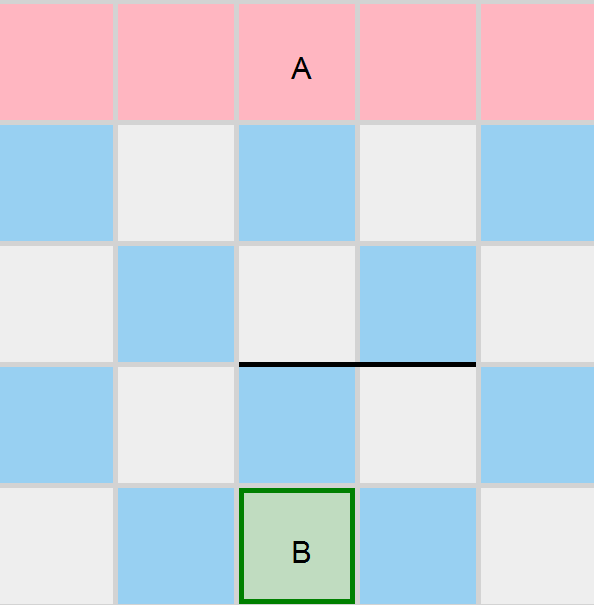
\includegraphics[width=\textwidth]{../img/GameBoard/wall_repr.png}
      \caption{Glendenning's Notation: \textbf{c3h}}
      \label{fig:NotationDifferentA}
    \end{subfigure}
    \hfill
    \begin{subfigure}{0.4\textwidth}
      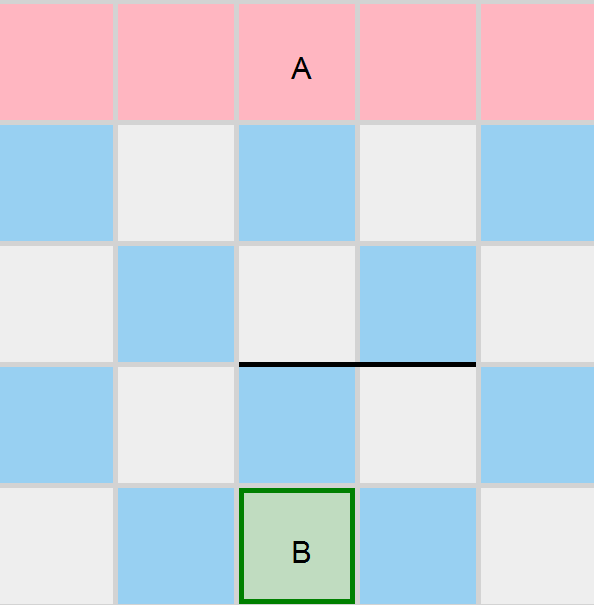
\includegraphics[width=\textwidth]{../img/GameBoard/wall_repr.png}
      \caption{Quoridor Strats Notation: \textbf{c4h}}
    \end{subfigure}
    \caption{Notation differences}
    \label{fig:WallNotationsDifferent}
\end{figure}

As seen in Figure \ref{fig:WallNotationsDifferent}, the difference lies in the exact position of the reference point of the walls of the wall. In the reference square, there are 4 corners. The reference point for horizontal wall placement is always the left corners of the cell. However, the difference in the notations lie in fact that whether the reference left corner is the left upper corner or the left lower corner. In the Quoridor Strats Notation, the reference starting point of the wall  is defined by the lower-left corner of the sqaure whereas in the Glendenning's Notation, each wall starts from the upper-left corner of the square. This difference is exemplified in the figure \ref{fig:WallNotationsDifferent}. In Glendenning's Notation, the wall placement with reference to the square $C_{3, c}$ i.e., c3h is defined with respect to the lower left corer of the square $C_{3. c}$. In contrary, in the Quoridor Strats Notation, the wall placement with reference to the $C_{4,c}$ i.e., c4h, is defined with respect to the upper left corner of the cell $C_{4,c}$. Since the lower left corner of the cell $C_{3,c}$ and the upper left corner of the cell $C_{4,c}$ are the same, the wall placement due to the notation difference were the same as seen in the figure.

Even though there notations are widely used, they are very easy to get confused with since they have the same wall representations,
and unless specified explicitly, it is difficult to tell which representation is being used. This ambiguity in notation necessitates a new notations, in particular for the wall placement to remove any confusion. For this purpose, in this thesis, we introduce a new notation for the purpose, particularly, of wall placement representation as follows:

\begin{equation}\label{eqn:Wall2}
W(C_{ij}) = jiD \text{ , where, } i \in \mathbb{R}, j \in \mathbb{K} \text{ ,and, } D \in \{N, S, E, W\}    
\end{equation}

In this new notation, we increase the size of the set $D$ from horizontal and vertical representation to north, south, east and west representations indicated by the characters 'N', 'S', 'E' and 'W'. This ensures that instead of an ambiguous vertical and horizontal wall representation with  respect to a cell, we can now define the direction explicitly. This wall additionally also implies that the wall in the 'N' and 'S' direction covers the reference cell, i.e., $C_{i, j}$ and the cell right to the reference cell, i.e., $C_{i, j+1}$ where $j+1$-th column represents the column on the right of the $j$-th column. Similarly, the wall in the 'E' and 'W' directions implies that the wall covers the reference cell $C_{i, j}$ and the cell below the reference cell, i.e., $C_{i+1, j}$ where $i+1$-row represents the row below the $i$-th row.

Looking back at Figure \ref{fig:NotationDifferentA}, the walls can now be represented by \textbf{c4N}, i.e. a Northern wall from the cell $C_{4, c}$.

This notation provides an additional flexibility to represent the wall placement in the game and removes the ambiguity that may be present as we saw earlier.

\section {Rules}
In this section, we formally define the rules of the game Quoridor, in particular for the wall placement and player movement.

\subsection{Wall placement rules}
\label{WallRules}

\begin{itemize}
    \item The walls have to be placed in either vertical or horizontal manner and they cannot be placed diagonally.
    \item A placed wall must not completely block any player's path to victory. Each player must have at least
        one path to victory. For example, in Figure \ref{fig:ValidState}, the walls are placed in such a way that player A has a valid path towards the edge of the player B, in particular, to the cells $C_{5, a}$, $C_{5, b}$, $C_{5, c}$, $C_{5, d}$ and $C_{5, e}$. However, the wall placement in Figure \ref{fig:WallBlockingMove}, due to the placement of the wall \textbf{c3N}, the player A does not have a valid path towards the edge cells of player B. Hence, the move \textbf{c3N} would be classified as an invalid move.
    \item A placed wall cannot intersect any of the previously placed walls. For example, in Figure \ref{fig:ValidState}, a walls has been placed with the moves \textbf{a1W}. A subsequent move \textbf{a2N} would be an invalid move in the game due as it requires the walls to intersect.
    \item Walls cannot be placed along the edges of the board. Walls must be placed to create a barrier for exactly 4 cells. For example, in Figure \ref{fig:ValidState}, a wall cannot be placed with the move \textbf{a1E} as it would only touch 2 cells $C_{1, a}$ and $C_{2, a}$ as it is on the edge of the board.
    \item  Every player possesses a limited supply of walls, and once they exhaust these walls, they are unable to place any additional ones. Consequently, in such situation the player is only allowed to maneuver their pawn on the
        board.
\end{itemize}

\begin{figure}[!ht]
    \begin{subfigure}{0.4\textwidth}
      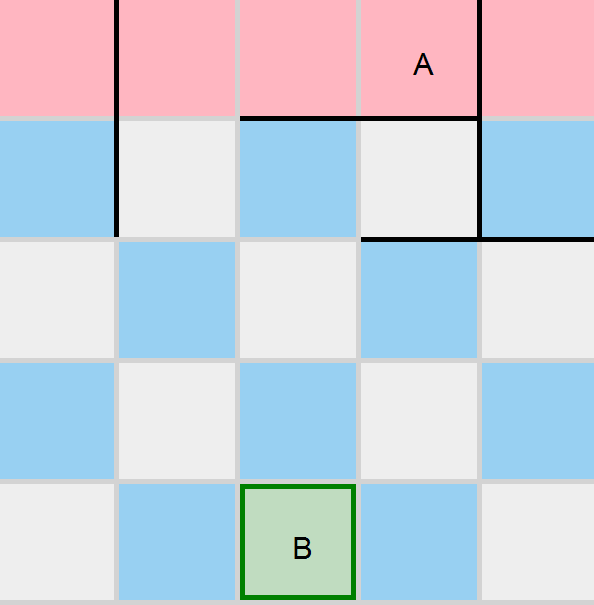
\includegraphics[width=\textwidth]{../img/GameBoard/arbitrary_state.png}
      \caption{Valid game state}
      \label{fig:ValidState}
    \end{subfigure}
    \hfill
    \begin{subfigure}{0.4\textwidth}
      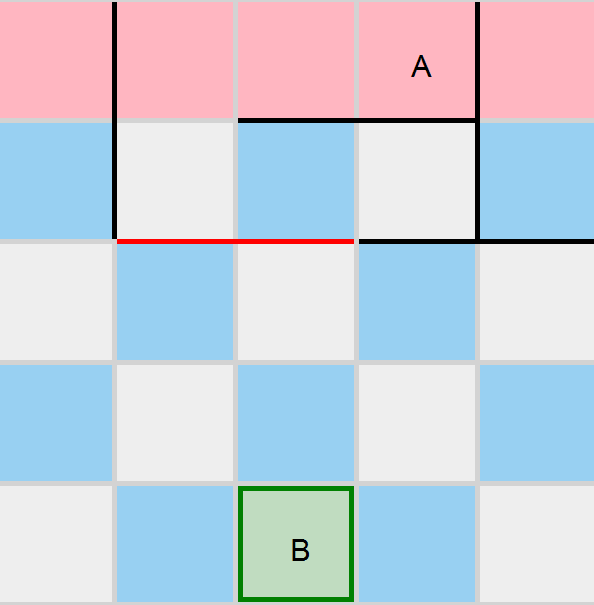
\includegraphics[width=\textwidth]{../img/GameBoard/invalid_wall.png}
      \caption{Invalid wall \textbf{b2S}}
      \label{fig:WallBlocked}
    \end{subfigure}
    \caption{Example of an invalid wall placement}
    \label{fig:WallBlockingMove}
\end{figure}

The game state represented by Figure \ref{fig:ValidState} shows the situation after 5 turns, with it currently
being player B's turn to move. Since both \textbf{A} and \textbf{B} have viable paths to their respective goal
rows and all walls have been placed according to the rules (see \textit{Section \ref{WallRules}}),
the game state shown in Figure \ref{fig:ValidState} is considered valid.
\par
However, player B disrupts the rules by placing the red wall, violating the specified wall-placement rules
(see \textit{Section \ref{WallRules}}), consequently rendering the game state represented by
Figure \ref{fig:WallBlocked} invalid.

\subsection{Player movement rules}
\label{PlayerMoveRules}
\begin{itemize}
    \item Players are allowed to move their pawn one cell at a time in the North, South, East, or West directions during their turn given that there is a cell and the cell is empty in the direction. Diagonal movements are not allowed. For example, a pawn in a cell $C_{2, c}$ can move to either in the north direction (i.e., $C_{1, c}$), the south direction (i.e., $C_{3, c}$), the west direction (i.e., $C_{2, d}$) or in the east direction $C_{2, b}$ given that the adjacent cells or squares empty. However, a pawn in the cell $C_{1,a}$ can only move in the west (i.e., $C_{1,b}$) and the south (i.e., $C_{2,a}$) direction as there are no squares on the east or the north of the cell.

    \item \textbf{Jump}
    \begin{itemize}
        \item If an opponent is at to the cell a player intends to move in the same direction of the opponent, the player can jump over the opponent provided there is no wall between the opponent or behind the opponent they intend to jump over. For example, in the first picture in figure \ref{fig:PossibleMoves} the player B can move to either of the squared highlighted in green. The player can move to east, west or south direction or can jump in the north direction over the player A from square $C_{4,c}$ to the square $C_{2,c}$ as there are no walls between the squares $C_{4,c}$, $C_{3,c}$ or $C_{2,c}$.
        
        \item If there is a wall between the opponent and the jumping square, the player can jump to a cell on either side of the opponent's cell, given the cell is accessible from the opponent's cell (i.e., there are no walls). In the section picture from left in the figure, for example, the player B cannot jump over player A to the cell $C_{2, c}$ due to the wall placement \textbf{c3N}. The player in this case can jump over to the cells on either the east side (i.e., cell $C_{3, b}$) or the west side (i.e., cell $C_{3, d}$) of the player A given there are no walls in between $C_{3, c}$ and $C_{3, b}$, and $C_{3, c}$ and $C_{3, d}$ respectively.
            
        \item Players cannot jump over walls. If a player is jumping from a cell $C_{1,*}$ to cell $C_{3,*}$, this is only possible if there are no walls in between them.
    \end{itemize}
\end{itemize}

\begin{figure}[!ht]
    \begin{subfigure}{0.2\textwidth}
      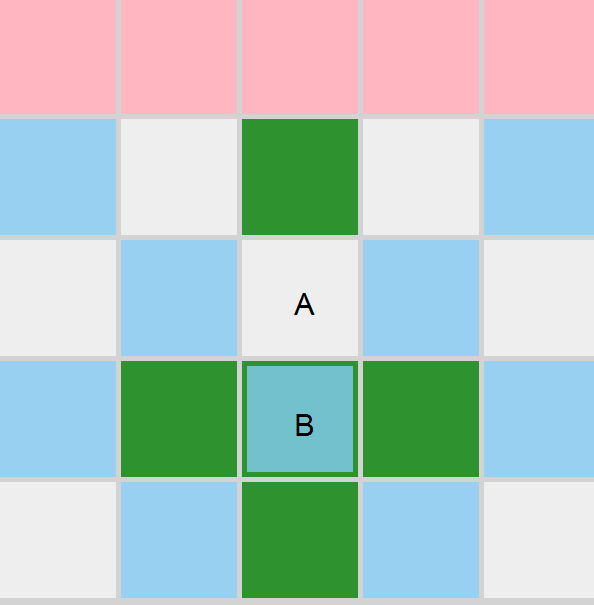
\includegraphics[width=\textwidth]{../img/GameBoard/move01.png}
    \end{subfigure}
    \hfill
    \begin{subfigure}{0.2\textwidth}
        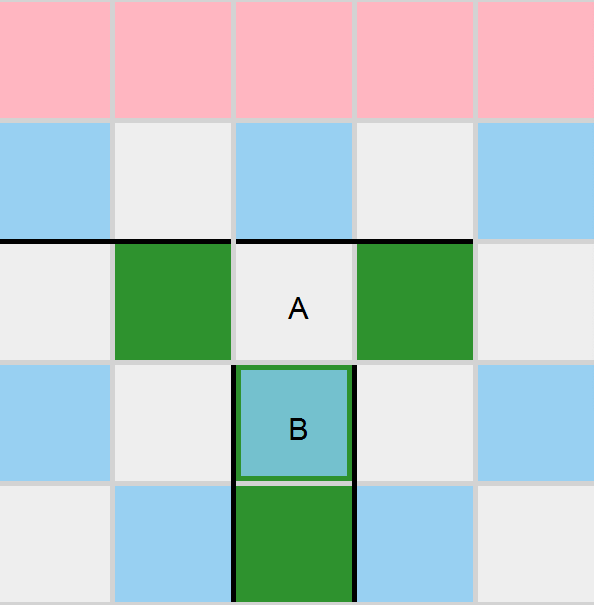
\includegraphics[width=\textwidth]{../img/GameBoard/move02.png}
    \end{subfigure}
    \hfill
    \begin{subfigure}{0.2\textwidth}
        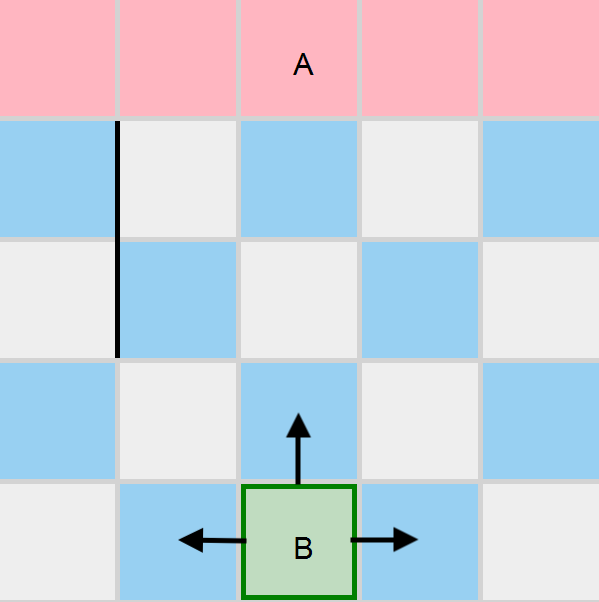
\includegraphics[width=\textwidth]{../img/GameBoard/move03.png}
    \end{subfigure}
    \hfill
    \begin{subfigure}{0.2\textwidth}
        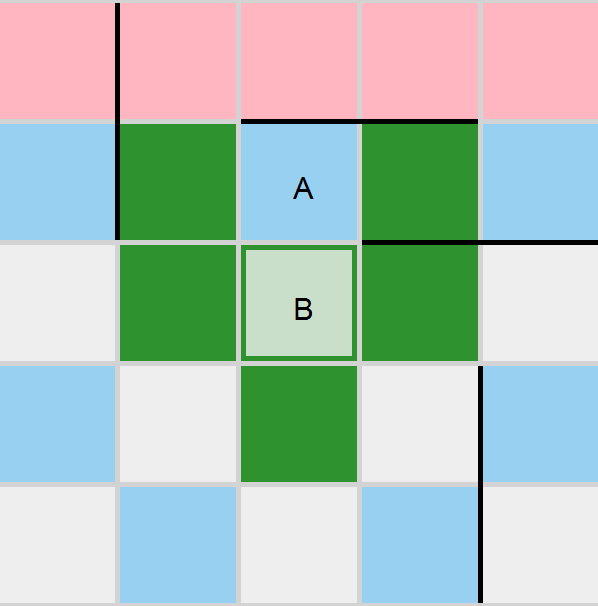
\includegraphics[width=\textwidth]{../img/GameBoard/move04.png}
    \end{subfigure}
    \caption{Examples of possible moves (marked green) for player B in different game states}
    \label{fig:PossibleMoves}
\end{figure}
\chapter{Related Works}\label{relatedworks}

Compared to some other strategy games such as Chess and Go, Quoridor has not been extensively studied in the literature. The authors in \citep{Brenner2015Artificial} developed an \gls{MCTS} approach for Quoridor. Recently, in \citep{Iwanaga2022Analysis}, the authors performed an analysis of the game for a miniature 5 by 5 board.

For this thesis, we consider the following works as our inspiration:

\begin{itemize}
    \item \textbf{Mastering Quoridor \citep{Glendenning2002MasteringQ}}\\
    The author of the thesis paper and assesses various algorithms like Negamax, Alpha-beta Negamax among others. Additionally, they utilized a genetic algorithm to refine the weights within a linear weighted evaluation function, employing 10 distinct features suggested by the author, some of which include player's position towards their goal side, the opponent's position towards their respective goal, the remaining count of walls available to the player, etc.

    \item \textbf{A Quoridor-playing Agent \citep{Mertens2006Quoridor}}\\
    The author of this paper delves deep into the theoretical aspects of Quoridor, providing an upper-bound on the state-space and the game-tree complexities, which we use as a foundation in Chapter \ref{GameAnalysis}.
    Furthermore, they also develop a Quoridor playing agent based on the Minimax algorithm.
    
\end{itemize}

In sharp contrast to the aforementioned works, our thesis takes a distinctly different path by delving deeply into the architectural aspects of AI. Our approach emphasizes abstraction to the greatest extent possible, with an eye on facilitating seamless integration into a broad spectrum of games. We prioritize creating an interface that is adaptable to diverse game environments, setting our research apart from the game-specific focus of the prior works.
\chapter{Game Analysis}
\label{GameAnalysis}

In Chapter \ref{GameDescription}, we explored the rules and gameplay mechanics of Quoridor.
As we progress, this chapter aims to deepen our understanding by analyzing Quoridor from a
theoretical and computational perspective.

In this chapter, we will classify Quoridor within the realm of strategic games, examine its game tree,
state-space and tree complexity, and explore the implications of these factors on gameplay and
artificial intelligence application.

\section{Classification of Quoridor}

Quoridor can be characterized as a discrete, deterministic, zero-sum, sequential, game with perfect
information \citep{Glendenning2002MasteringQ}, and therefore, a combinatorial game \citep{GameTheoryBook}. 

\subsection{Discrete}
In every turn of the game, each player has a finite number of moves and wall placements. These are limited by the game state (already placed walls and moved pawns) and the rules of the game. The game-tree of Quoridor has finite number of nodes (e.g Figure \ref{fig:GameTree}).

\subsection{Deterministic}
Quoridor has no random elements or chance involved in the gameplay. Every outcome is a direct result of the players' strategies and the subsequent decisions. As there is no random aspect to the game, hence, this is a deterministic game.

\subsection{Zero-sum}
In Quoridor, when a player makes a move that brings them closer to winning (like advancing their pawn or placing a wall effectively), it inherently puts the opponent at a disadvantage. Therefore, any positive progress for a player translates into a negative impact for their opponent. This reciprocal relationship of gain and loss between the players is what characterizes Quoridor as a \textbf{zero-sum} game.

\subsection{Perfect Information}
Every aspect of its gameplay are completely visible and known to all players at all times. This means that the positions of the pawns and the placements of the walls on the board are always in full view, allowing players to make strategic decisions based on the entire state of the game. Hence, this property classifies the game as a game of perfect information.

\section{Game-Tree}

A game tree for an abstract-strategy game (discrete games with perfect information) is a comprehensive graph representing every possible game states and sequence of moves. The nodes of a game tree represent game states, and the edges represent actions/moves.

Game trees are integral to the framework of adversarial search problems, where they are employed to systematically explore and evaluate the possible outcomes of different strategies, and forecast future states of the game based on current and potential moves.

\begin{figure}[!ht]
    \centering
    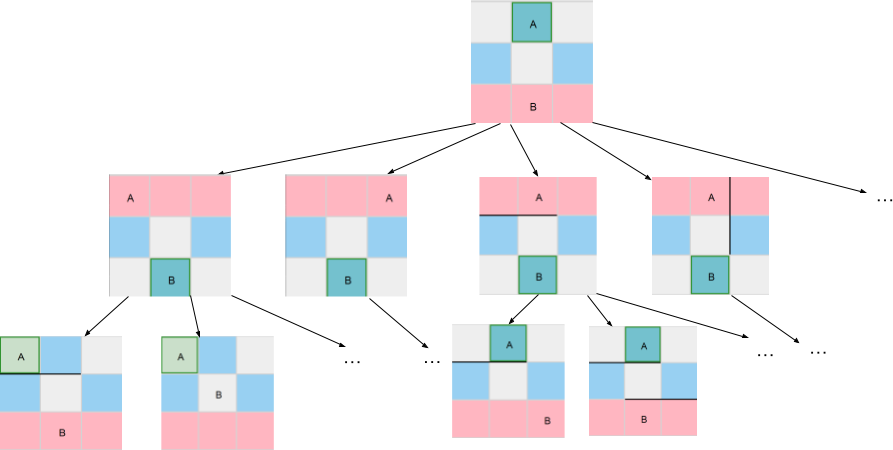
\includegraphics[scale=0.45]{../img/GameBoard/game_tree.png}
    \caption{A partial game tree for a 3x3 game board.}
    \label{fig:GameTree}
\end{figure}

As depicted in Figure \ref{fig:GameTree}, the root node of the game tree consists of player A located in the cell $C_{1, b}$ making a choice for the first move which may be one of pawn movement or wall placement. The nodes at a depth of 1 represent all possible game states as a result of moves made by player A and so on.


\subsection{Branching Factor}
\label{BranchingFactor}

The branching factor of a Game-tree is the number of child nodes of each node, or in other words, the number of possible moves a player at their turn can make, given the game state.

In Figure \ref{fig:GameTree}, player A makes the first move. A has \textbf{3} places to move their pawn to and \textbf{8} places to put one of their walls at. So, the root node has a branching factor of \textbf{11}.

The branching factor is greatly influenced by the state of the board in Quoridor, i.e the location of the pawn of the player, the location of the pawn of the opponent and the walls placed on the board.

As an example, the figure below represents a game states with the maximum and minimum branching factors:

\begin{figure}[!ht]
    \begin{subfigure}{0.4\textwidth}
      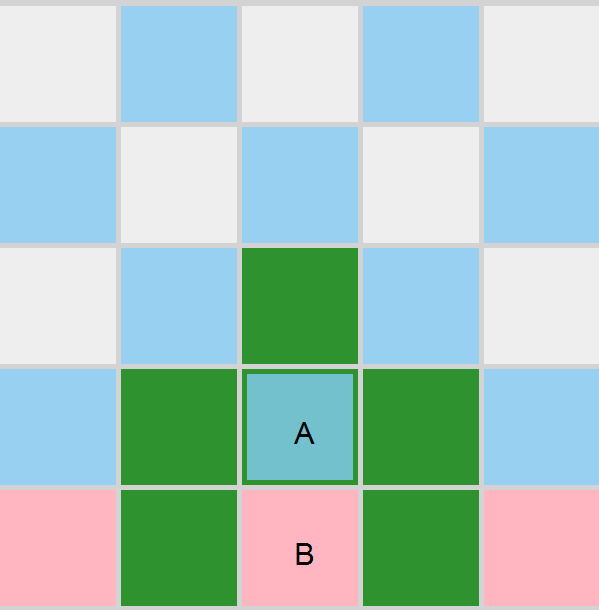
\includegraphics[width=\textwidth]{../img/GameBoard/maximum_branching_factor.png}
      \caption{Maximum : 37}
      \label{fig:MaxBranchingFactor}
    \end{subfigure}
    \hfill
    \begin{subfigure}{0.4\textwidth}
      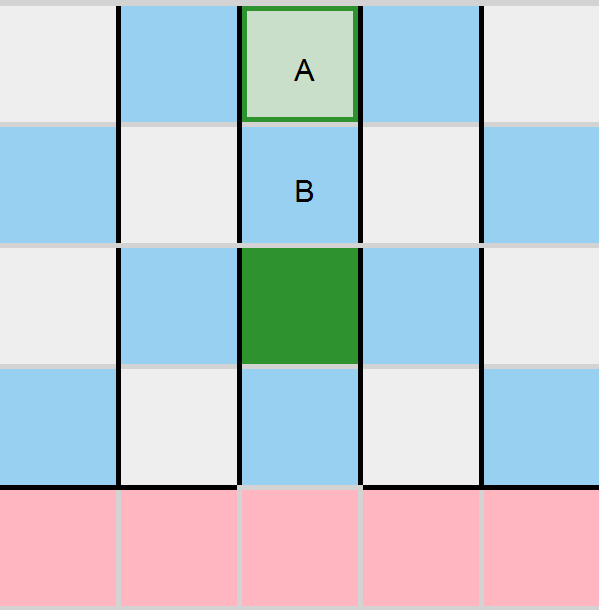
\includegraphics[width=\textwidth]{../img/GameBoard/minimum_branching_factor.png}
      \caption{Minimum : 1}
        \label{fig:MinBranchingFactor}
    \end{subfigure}
    \caption{Branching factor differences}
\end{figure}

As depicted by Figure \ref{fig:MaxBranchingFactor}, player A has 5 possible places to move their pawn to. No walls have been placed so far, so player A can also place one of their walls in any groove.

For a board of size NxN with no walls placed, $N-1$ walls can be placed in each row (since each wall occupies 2 cell lengths), and there are $N-1$ rows for correct horizontal wall placements. Hence, there are $(N-1)^2$ slots for horizontal wall placements, and since the board is NxN, the total  slots for both horizontal and vertical wall placements is given by the equation:
\begin{equation}
\label{eq:WallPlacements}
    2(N-1)^2
\end{equation}

Coming back to Figure \ref{fig:MaxBranchingFactor}, since the board has no walls placed, we now see that A has $5 + 2(5-1)^2 = 37$ possible moves they can perform, ergo, the branching factor of the game state represented by Figure \ref{fig:MaxBranchingFactor} is \textbf{37}, which is also the maximum branching factor for board sized 5x5.

However, in Figure \ref{fig:MinBranchingFactor}, player A has no available slot for wall-placement, and the already-placed walls block A from moving anywhere except for cell \textbf{$C_{3, c}$}. Hence, the branching factor for the game state represented by Figure \ref{fig:MinBranchingFactor} is \textbf{1}.

\subsubsection{Average Branching Factor}

In Sub-Section \ref{BranchingFactor}, we saw that the branching factor is not uniform due to factors like wall-placements and positioning of players greatly influencing it.

We, therefore, would like to estimate an average branching factor for boards of different dimensions to see if varying board dimension has any effect in the average branching factor.

We already know from Equation \ref{eq:WallPlacements} that the maximum branching factor of the game tree is exponential in order of $N$ and from Figure \ref{fig:MinBranchingFactor}, we can deduce that the minimum branching factor is 1 (since we can replicate a similar game state for any dimension).

To find an estimate of the average branching factor $B_{avg}$, we propose Algorithm \ref{alg:AverageBranchingFactor}, which runs N simulations between 2 agents, keeping a track of the total game states encountered and the total moves made by agents, and averaging their values.

\begin{algorithm}[!ht]
\caption{Average branching factor}
\label{alg:AverageBranchingFactor}
\DontPrintSemicolon
\SetKwInOut{Input}{input}\SetKwInOut{Output}{output}
\SetKwFunction{FMain}{AvgBranchingFactor}
\SetKwProg{Fn}{Function}{:}{}
\Fn{\FMain{agent1, agent2, simulations}}{
    \Input{Two agents and number of simulations}
    \Output{Average branching factor}
    SumOfAverages $\gets$ 0\;
    \For{i $\gets$ 1 \KwTo simulations}{
        State $\gets$ Initialize()\;
        GamePossibleMoves $\gets$ 0\;
        GameMovesMade $\gets$ 0\;
        Agents $\gets$ [agent1, agent2]\;
        AgentIndex $\gets$ 0\;
        \While{State is not Terminal}{
            Agent $\gets$ Agents[AgentIndex]\;
            AgentIndex $\gets$ (AgentIndex + 1) \% 2\;
            GamePossibleMoves $\gets$ GamePossibleMoves + Length(State.PossibleMoves())\;
            Move $\gets$ Agent.GetMove(State)\;
            State $\gets$ State.Apply(Move)\;
            GameMovesMade $\gets$ GameMovesMade + 1\;
        }
        GameAverage $\gets$ GamePossibleMoves / GameMovesMade\;
        SumOfAverages $\gets$ SumOfAverages + GameAverage\;
    }
    \KwRet SumOfAverages / simulations\;
}
\end{algorithm}

We then simulate \textbf{1000} games between \textbf{Minimax} and \textbf{Semi-random} agents, each for boards of dimensions 3, 5, 7 and 9, and for depths 1, 2 and 3, and the results of the average branching factor can be seen in Figure \ref{fig:BranchingFactor}.

\begin{figure}[!ht]
    \centering
    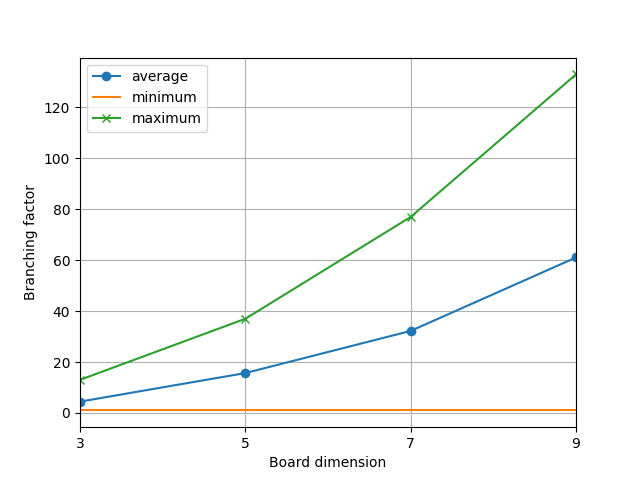
\includegraphics[scale=0.6]{../img/branching_factor.png}
    \caption{Branching factor for boards of different sizes}
    \label{fig:BranchingFactor}
\end{figure}

From Figure \ref{fig:BranchingFactor}, like with the maximum branching factor, we can see a similar exponential trend of the average branching factors in order of $N$. Furthermore, based on only the four dimensions and their averages and maximum branching factors, the average branching factor seems to be almost half the maximum branching factor.

The average branching factor for board of dimension 9x9 was about \textbf{61}, which is very close to the value proposed by \citep{Glendenning2002MasteringQ} which was 60.

\section{State space complexity}

The state space complexity is a measure of a game complexity and refers to the total number of possible states in a game. For example, for illustration with the game of Tic-Tac-Toe, there are 9 squares, each being one of X, O or empty. The state space complexity for Tic-Tac-Toe can be written as $3^9 = 19,638$. Of course, this takes into account the illegal positions as well such as all Xs or all Os and hence can be considered as an upper bound on the state space complexity. However, especially in complex games such as Chess and Quoridor with many possible states, rules and illegal positions, exact state space complexity is difficult to estimate and a way to define the complexity is through an upper bound.  

In Quoridor, this includes all the possible positions of both players' pawns on the board and all the possible configurations of walls. It is extremely difficult to find an exact value because we also need to account for wall placement rules \ref{WallRules} and pawn movement rules \ref{PlayerMoveRules}. Because of this, we loosen the regulations to come up with an upper-bound.

In \citep{Mertens2006Quoridor}, the author has determined the state space complexity for a specific board of dimension 9x9. In this thesis, we generalize the complexity evaluation to a general board of size NxN.

For a board of Dimension NxN, the first pawn can be placed in $N^2$ possible locations. After the first pawn is placed in the board, the second pawn now has $N^2-1$ possible locations to be placed into. So, the total number of ways for pawn placement, $S_p$ is given by
\begin{equation}
    S_p = N^2(N^2 - 1)
\end{equation}

As for walls, from Equation \ref{eq:WallPlacements}, we know that there are $2(N-1)^2$ ways of placing walls on the board, both horizontally and vertically. Since we know that each wall occupies 2 cells, we will use assumption made by the author of \citep{Mertens2006Quoridor} that placing the wall anywhere in the board takes away the possibility of placing walls at 4 different places. As each placed wall takes two cells, placing a wall, for e.g., horizontally, means that further walls cannot be placed in the location of the wall, walls starting from the cell left and right to the cell of the wall and a wall placed vertically through the placed wall. Every placed wall hence takes away 4 spaces for wall placement. The same example is also valid for a vertically placed wall. Hence assuming that $j$ walls are placed from a given game state, the total number of branches of the game state for wall placement may be $2(N-1)^2 - 4j$,

Furthermore, for a given board dimension (e.g., NxN), there is a fixed number of walls in the game $N_w$. For example, for the standard 9x9 board with 81 total squares, $N_W = 20$. We can extrapolate the number of walls that may be available for boards of other dimensions too based on the number of squares. For example, for 3x3 board, $N_W = 2$, for 5x5 board $N_w = 8$, for 7x7 board $N_W = 12$.

In the game tree, there may be a path where a total of $N_W$ walls are used. In such scenario, the total number of branches $L_{N_w}$ in the tree can be defined by the following equation:
\begin{equation}
    L_{N_w} = \prod_{j=0}^{N_w} (2(N-1)^2 - 4j),
\end{equation}
where, each component in the product defines the total number of states in the subsequent turn following a wall placement.

However, in the game, all the walls may not be necessarily placed. Hence, in such case, the total number of walls used may be variable and hence the total possibilities for wall placement $S_w$ is defined by the following equation:
\begin{equation}
    S_w = \sum_{i=0}^{N_w}\prod_{j=0}^{i}(2(N-1)^2 - 4j).
\end{equation}

And thus, since the game tree consists of the possibilities of both pawn movement and wall placement, the total state space complexity is given by $S = S_w * S_p$. \citep{Mertens2006Quoridor}

\begin{equation}
    S = N^2(N^2 -1) \times \sum_{i=0}^{N_w}\prod_{j=0}^{i}(2(N-1)^2 - 4j).
\end{equation}

\begin{figure}[!ht]
    \centering
    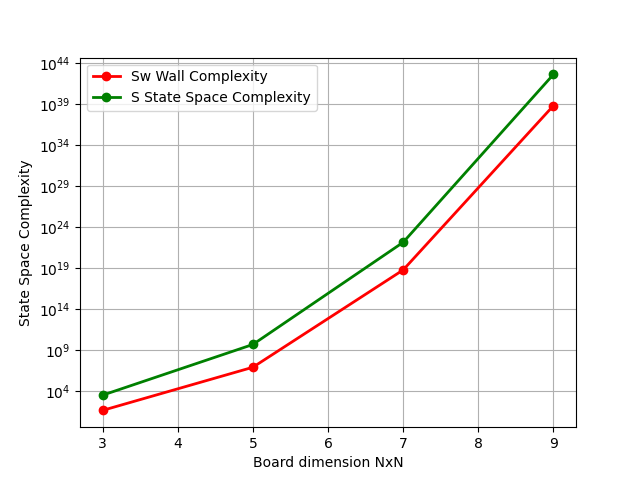
\includegraphics[width=.9\linewidth]{../img/Complexity.png}
    \caption{Complexity vs Board Dimension}
    \label{fig:complexity}
\end{figure}

In Figure \ref{fig:complexity}, we can see the log plot of the state space complexity of wall placement and the game when varied with the dimension of the game (i.e., 3x3, 5x5, 7x7 and 9x9). In the figure, we can see the state space of the game grows exponentially with the increase in the board dimension. Moreover, the state space complexity is dominated by the complexity of the wall placement as seen by the difference between the two curves.


\section{Game tree complexity}

The game-tree complexity of a game, as defined in \citep{Allis1994Searching}, is another measure of a game complexity alongside the state-space complexity. The authors define a game tree complexity as "\textit{the number of leaf nodes in the solution search tree of the initial position(s) of the game}".

The game tree complexity refers to the number of possible games that can be played. Unlike the state space complexity, which measures the total number of possible states of the game from the starting position, the game tree complexity measures the size of the game tree. The size of the game tree or the game-tree complexity typically is larger than the state space complexity because a game state (counted only once in the state space complexity) can arise through multiple games (counted multiple times in the game tree complexity).

An example of the game tree complexity can be illustrated through the game of tic-tac-toe. In the game tree, player A has 9 positions to put the mark (e.g., X or 0) on. Subsequently, in the second move, player B can put the mark on 8 spaces as one has been taken away in the first move and so on. Hence, the game tree complexity of tic-tac-toe can be defined as $9 \times 8 \times \cdots \times 1 = 9! = 362380$. In comparison to the state space complexity of tic-tac-toe, the game tree complexity is higher as a position arising through different orders of play is counted as one state with the state space complexity and multiple game tree positions with the game tree complexity. 


In complex games like Quoridor, the game-tree complexity $G$ can be estimated by raising the average branching factor $B_{avg}$ to a power of the total number of moves by the players $D_{avg}$ \citep{Mertens2006Quoridor}, which is given by the following equation: 
\begin{equation}
    G = B_{avg}^{D_{avg}}
\end{equation}

The average depth $D_{avg}$ simulated for different dimensions of the game can be found below:
\begin{align*}
    &D_{avg, \text{3x3}} = 11\\
    &D_{avg, \text{5x5}} = 47\\
    &D_{avg, \text{7x7}} = 72\\
    &D_{avg, \text{9x9}} = 97
\end{align*}

Subsequently, we can now determine the game tree complexity based on the determined $B_{avg}$ and $D_{avg}$. The game tree complexity for different dimensions can be written as:
\begin{align*}
    &G_\text{3x3} = 8.58 * 10^9\\
    &G_\text{5x5} = 9.94 * 10^{58}\\
    &G_\text{7x7} = 5.56 * 10^{113}\\
    &G_\text{9x9} = 1.50 * 10^{173}
\end{align*}

From this, we can infer that the game state complexity for Quoridor, like the state space complexity, also increases exponentially with the increase in the dimension of the game.


\section{Comparison with other games}

\begin{table}[ht]
    \centering
     \begin{tabular}{|c|c|c|c|}\hline
          & $\log_{10}(S)$ & $\log_{10}(G)$ & $B_{avg}$\\ \hline 
          Tic-tac-toe  & 3   & 5   & 4    \\ \hline
  \textbf{Quoridor 3x3} & 3  & 10  & 8  \\ \hline
          Connect-four & 13  & 21  & 4    \\ \hline
  \textbf{Quoridor 5x5} & 10  & 59 & 18  \\ \hline
  \textbf{Quoridor 7x7}  & 22  & 113 & 38  \\ \hline
          Chess        & 44  & 123 & 35   \\ \hline
  \textbf{Quoridor 9x9}     & 42  & 173 & 61  \\ \hline        
          Go           & 170 & 360 & 250 \\ \hline
     \end{tabular}
     \caption{State space, game tree and branching factor comparison between well-known games}
     \label{tab:comparison}
 \end{table}

 In the Table \ref{tab:comparison}, we present the logarithm of the state space complexity ($\log(S)$), the game state complexity ($\log(G)$) and the average branching factor ($B_avg$) of some popular games from the literature \citep{Mertens2006Quoridor}.

 As we can see from the above table, Quoridor with board dimension 3x3 has the state space complexity and the game tree complexity similar to that of Tic-tac-toe. It can also be inferred that the Quoridor game with dimension 9x9 has similar complexity compared to chess.
 
\chapter{AI agents}
\label{background}

In this chapter, we give a brief overview of different \gls{AI} techniques that have been considered for implementing the agent for Quoridor in this thesis including the Minimax algorithm, \gls{MCTS} and A-star algorithm.

\subsection{Minimax algorithm} \label{sec:minimax}
Minimax algorithm, first proven by John von Neumann in 1928 in his paper \textit{Zur Theorie Der Gesellschaftsspiele} \citep{v1928theorie}, is a very popular algorithm employed in many decision-making scenarios for e.g., in decision theory, game theory and even philosophy. As suggested by the name minimax, the idea of the algorithm is to minimize the player's loss when the opponent makes a decision that gives the player the maximum loss. This algorithm has been implemented in many multi-player strategy games such as Tic-Tac-Toe \citep{savelli2008tic}. 


Mathematically, a minimax algorithm can be defined by the following equation:
\begin{equation}\label{eq:mmax}
    \bar{v}_i = \min_{a_{-i}} \max_{a_{i}} v_i (a_i, a_{-i})
\end{equation}
where,
\begin{subequations}
\begin{align}
    &i, -i = \text{index of the player of interest, opponent respectively} \\
    &a_i, a_{-i}= \text{action of the player of interest, opponent respectively} \\
    &v_i = \text{value function of player i} \\
    &\bar{v}_i = \text{minimax value of the player of interest}
\end{align}
\end{subequations}

As defined in the Equation \eqref{eq:mmax}, the minimax algorithm comprises of two parts. The first part is maximizing part where the player chooses an action from a set of possible actions to maximize the evaluation of the game. Then, the player determines the subsequent action of the opponent to minimize the evaluation of the game. This is clarified further with the following example.

\begin{figure}
    \centering
    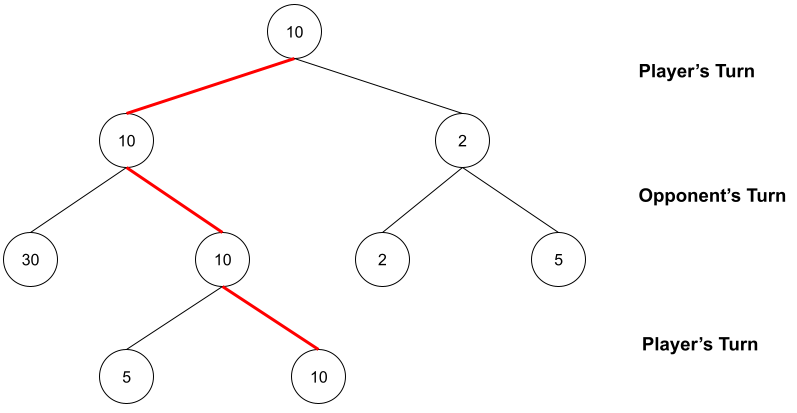
\includegraphics[width=\linewidth]{../img/Minimax1.png}
    \caption{Figure illustrating an exemplary game tree and decision based on minimax algorithm}
    \label{fig:minimax1}
\end{figure}

The Figure \ref{fig:minimax1} consists of nodes that define either player's or the opponent's actions. In our minimax implementation, we have considered an evaluation function as a linear combination of multiple features such as shortest distance to the goal and remaining number of walls. This is explained in detail in Section \ref{sec:gameimplementation}. The numbers for each node Figure \ref{fig:minimax1} represent the evaluation of this function. For each action, there can be an evaluation where higher evaluation may mean it is favouring the player. For example, an action of the player causing two possible evaluations of 10 and 20 would mean the player would have higher advantage choosing the action leading to evaluation of 20. 

The minimax algorithm starts with a game tree with possible moves of the player and opponent. The evaluation of the leaf nodes positions are assigned, for example 5 and 10 in the figure. The player chooses a move to maximize the evaluation on their turn whereas the opponent wants to minimize the evaluation. The player chooses evaluation of 10 (between 10 and 5) on its turn and subsequently evaluation of 10 (between 10 and 30) in the opponent's turn. The red line shows the path the player determines as optimal leading to a decision choosing the the action labelled with evaluation of 10.

The minimax algorithm involves in the player performing an exhaustive search on the game tree to determine a sequence of maximizing and minimizing moves. The complexity of such algorithm in large game tree often means such search is often impossible due to limited computational resources. To limit this complexity, further techniques such as depth-limited minimax, alpha-beta pruning and parallel minimax algorithm can be used.

\subsubsection{Alpha-beta pruning}

\begin{figure}[!ht]
    \centering
    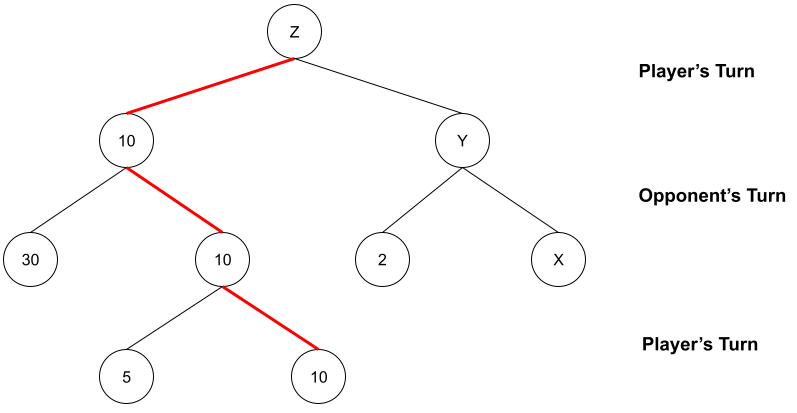
\includegraphics[width=\linewidth]{../img/Minimax2.png}
    \caption{Exemplary figure illustrating the alpha beta pruing for minimax algorithm}
    \label{fig:minimax2}
\end{figure}

Alpha-beta pruning is one way to reduce the compelxity of the minimax algorithm without affecting the performance of it.

In many cases, there may be the actions of the player in the search tree that can be evaluated worse than another action already evaluated. In such cases, where the better move or action has already been determined, it may not be useful to further evaluate the subsequent moves of the player and the opponent. Hence, the alpha-beta pruning reduces the game complexity by not further evaluating the branches of the node with evaluation worse than what has already been determined with another node.

As its name suggests, the alpha beta algorithm maintains two values, alpha and beta values. The alpha value stores the minimum score the player is assured to get while the beta value records the maximum score the opponent is assured to get. Whenever the evaluation of the minimum score of the player is higher than the maximum score after the subsequent move of the opponent (or in other words alpha $>$ beta), the alpha-beta pruning algorithm stops evaluating the opponents position. This reduces the number of nodes in the search tree and hence reduces the complexity of the minimax algorithm.

In Figure \ref{fig:minimax2}, if the player determines that 
\begin{equation}
    Z = max (10, Y) = max (10,  min (2, X)),
\end{equation}
the value of X does not influence the value of $Y$ or $Z$ as $Y = min(2, X) \leq 2$ and hence $Z = max(10, \leq 2) = 10$. In this case, the player may not evaluate the branch $X$ or branch $Y$ further reducing the game tree and hence the computational complexity of the algorithm. 

\subsubsection{Parallel minimax}
Another way to improve the time complexity of the minimax algorithm is to parallelize the algorithm. The minimax algorithm involves in evaluating multiple nodes of the game tree. The way to parallelize such algorithm is to run different processes, in this case, evaluation of the position associated with different nodes, in different threads. This ensures that even though computational complexity may remain the same, the time complexity of the algorithm is distributed over multiple threads and possibly multiple processors.


\subsection{Monte-Carlo Tree Search}\label{sec:MCTS}
\gls{MCTS} \citep{Coulom2006Efficient} is a heuristic tree search algorithm popular in decision-making processes, mostly popular in strategic games where the game tree space is too large to traverse. One problem with the minimax algorithm is that it requires a robust and accurate evaluation function to evaluate a given position in the game. This problem can be even more relevant when the game tree space is too large making it difficult to find the evaluation of a position. The basic idea of the \gls{MCTS} algorithm is that it narrows down on certain areas of the game tree, such that the exhaustive traversal search of the tree is not required. The algorithm achieves this by taking random samples in the tree space and building a search tree based on it.

\begin{figure}[!ht]
    \centering
    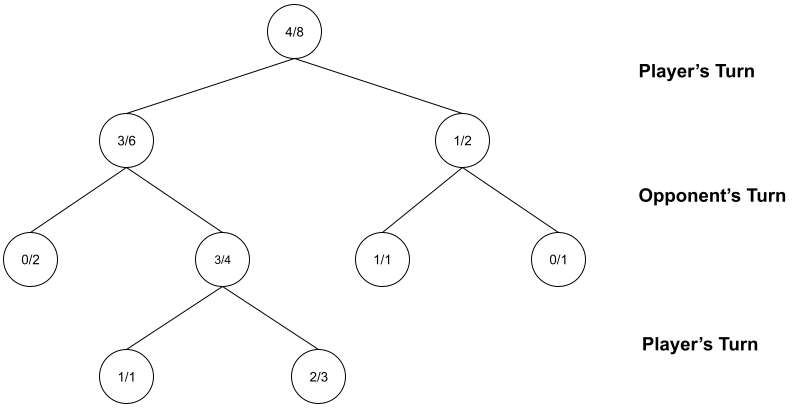
\includegraphics[width = \linewidth]{../img/MCTS1.png}
    \caption{Figure illustrating an iteration of the MCTS algorithm}
    \label{fig:MCTS1}
\end{figure}

As shown in Figure \ref{fig:MCTS1}, \gls{MCTS} algorithm determines the best path to the destination node in the game tree based on multiple trial runs through the game tree. In the figure, each node is labelled with a fraction where the denominator represents the total number of game runs through the node and the numerator represents the total number of wins for the player. For example, the game is simulated a total of 8 times in the example where the player wins 4 of the runs. The player wins 3/6 when taking an action while 1/2 when taking another action and so on.

The \gls{MCTS} algorithm builds upon the following framework:
\begin{enumerate}
    \item \textbf{Selection:} This step involves the algorithm choosing a move based on either a good move determined in previous iterations or a exploratory new move. The algorithm uses the Upper Confidence Bound for Trees \textbf{(UCT)} to guide this decision, balancing the tradeoff between exploration of uncharted nodes and exploitation of nodes with a high success rate.
    
    Mathematically,
    \begin{equation}
        UCT(n) = \overline{X}(n) + c U(n)
    \label{eq:UCT}
    \end{equation}
    where,
    \begin{subequations}
    \begin{align}
        \overline{X}(n) = \text{average win rate of node n} \\
        U(n) = \sqrt{\frac{\ln{N(P(n))}}{N(n)}   }
    \end{align}
    \end{subequations}
    
    
    \item \textbf{Expansion:} This step involves the algorithm to add a new node to the game tree determined during the selection process. A node can simply be a valid move starting from the node from where no simulation step has been played out. In Figure \ref{fig:MCTS2}, an un-evaluated option (e.g., node inside the dotted box) is explored and simulated.
    \item \textbf{Simulation:} This step involves the agent playing out the game using policy. One of the policies can simply be a random policy (e.g., choosing a move based on certain distribution).
    \item \textbf{Back propagation:} Finally, based on the simulation step, this step involves in the algorithm updating the nodes. In Figure \ref{fig:MCTS2}, the red arrows show the back propagation step as a result of exploration and simulation step where the probabilities or the weights of the nodes are updated as a result of exploration and simulation steps.
\end{enumerate}

\begin{figure}[!ht]
    \centering
    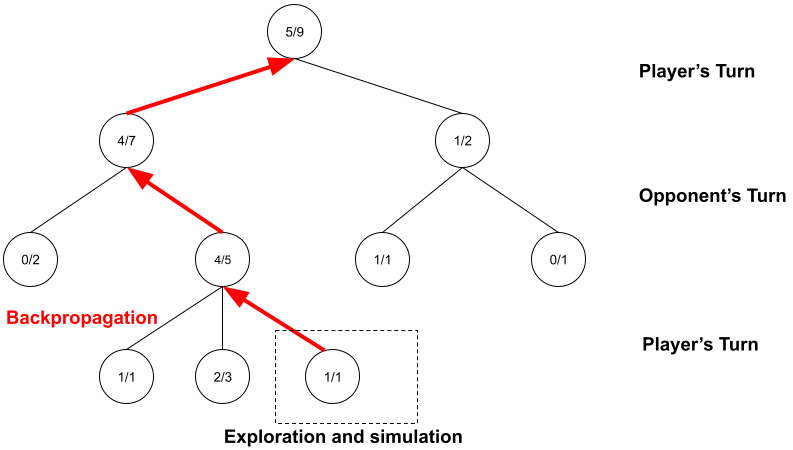
\includegraphics[width=\linewidth]{../img/MCTS2.png}
    \caption{Figure illustrating steps 2, 3, and 4 of the MCTS algorithm}
    \label{fig:MCTS2}
\end{figure}

The advantage of \gls{MCTS} algorithm over the minimax algorithm is that the \gls{MCTS} algorithm does not require any evaluation function as the weights are determined based on multiple simulation runs. On the contrary, the \gls{MCTS} algorithm requires multiple runs through the game to determine the weights.





\subsection{A-star algorithm}
A star is a popular algorithm \citep{Hart1968AFormal} used mainly for graph search and traversal problems. The main aim of the A-star algorithm is to find a path between a starting node and an destination node with the least cost. The cost function of the algorithm comprises of two components, the distance from the starting node to the current node and the estimated heuristic from the current node to the destination node. As the distance to the destination node may not be exactly known, one may use the estimate such as Manhattan distance and Euclidean distance. In the context of Quoridor gameplay, for example, we use the \textit{Manhattan} heuristic (see Equations \ref{eq:playerPHeuristic} and \ref{eq:playerQHeuristic}).

The cost function, or "f" score, for a node depends on two components "g" value and "h" value. "g" value represents the distance from the source node to the node and "h" value represents the cost of the path from the node to the destination node, often defined by a heuristic. Mathematically,
\begin{equation}
    f = g + h
\end{equation}
\chapter{Implementation}\label{Implementation}

In this chapter, we delve into the practical aspects of creating \gls{AI} agents capable of tackling abstract strategy games. The focus is on constructing adaptable interfaces that can be applied to a variety of games, ranging from the simplicity of Tic-tac-toe to the profound strategic depths of Go, with our primary case study being the game of Quoridor.

\gls{Csharp}, is selected as the language of choice, mainly for its robustness, versatility, and strong support for object-oriented programming paradigms. \gls{Csharp}'s rich feature set makes it an excellent tool for developing sophisticated \gls{AI} frameworks that require a blend of performance, maintainability and readability.

\section{Interfaces}
\label{game_interface_def}
The architecture of our implementation leverages interfaces, which specify a set of methods relevant to game mechanics. They form the backbone of our \gls{AI} systems, ensuring that the algorithms are versatile and can be adapted to new games with minimal changes to the underlying codebase. An example of such interface usage can be seen in Section \ref{TicTacToe}

Through the use of generic parameters \textbf{TPlayer}, \textbf{TMove}, and \textbf{TGame}, these interfaces offer a framework that is adaptable to various game entities such as players, moves, and game states.

Before describing the game-specific interfaces, we first introduce the generic interface \textbf{IAIStrategy\textless{}TMove, TGame, TPlayer\textgreater{}}, which acts as a common interface for all our \gls{AI} agents.
\begin{lstlisting}
interface IAIStrategy<TMove, TGame, TPlayer>
{
    string Name { get; }
    
    AIStrategyResult<TMove> BestMove(
        TGame game, TPlayer player);
}

class AIStrategyResult<TMove>
{
    double Value { get; set; }
    TMove BestMove { get; set; }
}
\end{lstlisting}
This interface provides a common property \textbf{Name}, a \texttt{string} representing the name of the agent, and a method \textbf{BestMove} that takes in a game and the current player in the game, and returns a tuple - the first item labelled as \textbf{BestMove} (parametrized over generic type \textbf{TMove}) being the best move for the current player in the given game state and the second item of the tuple labelled as \textbf{Value}, a \texttt{double} type representing the value corresponding to the best move selected by the \gls{AI} agent.
For example, for the Minimax algorithm, the Value corresponding to the best move would be the state with the highest payoff function, which could be used for debugging purposes.
\\
The following interfaces are used within the \textbf{BestMove} method for each \gls{AI} agent, and are meant to be defined explicitly by the user within their game.

\subsubsection{IValidMoves}

\begin{lstlisting}
interface IValidMoves<TMove>
{
    IEnumerable<TMove> GetValidMoves();
}
\end{lstlisting}

The \textbf{IValidMoves\textless{}TMove\textgreater{}} interface is the most fundamental interface used by (almost) all our \gls{AI} systems. Parametrized over the generic type \textbf{TMove}, this interface provides access to all valid moves (of a user-defined \textbf{TMove} type), e.g from the current game state, which our implemented \ac{AI} algorithms evaluate and find the best move.

\subsubsection{IPlayer and IOpponent}

\begin{lstlisting}
interface IPlayer<TPlayer>
{
    TPlayer CurrentPlayer { get; }
}

interface IOpponent<TPlayer>
{
    TPlayer Opponent { get; }
}
\end{lstlisting}

Since we are focused on abstract two-player games, we also provide the \textbf{IPlayer\textless{}TPlayer\textgreater{}} and \textbf{IOpponent\textless{}TPlayer\textgreater{}} interfaces, both parametrized over the generic \textbf{TPlayer} type.
The \gls{MCTS} algorithm, for example, uses these interfaces during the simulation and back-propagation phases.

\subsubsection{IDeepCopy}

\begin{lstlisting}
interface IDeepCopy<T>
{
    T DeepCopy();
}
\end{lstlisting}
Although \gls{Csharp} has the \textbf{ICloneable\textless{}T\textgreater{}} interface provides a \textbf{T Clone()} method that we could use instead of our defined \textbf{IDeepCopy\textless{}T\textgreater{}} interface, the method we define leaves no room for ambiguity on shallow vs deep copying of relevant objects.
This method is used by e.g the Parallel Minimax algorithm in order to ensure the original game state don't get changed by any means while exploring the game tree by making several moves.

\subsubsection{ITerminal}

\begin{lstlisting}
interface ITerminal
{
    bool HasFinished { get; }
}
\end{lstlisting}
Another important information for a game is whether the game reached the terminal state (win, loss, draw). This information helps update evaluations of game states and also notifies the algorithms to stop looking further. For example, the Simulation step of the \gls{MCTS} algorithm performs moves until the game reaches a terminal state.

\subsubsection{IStaticEvaluation}

\begin{lstlisting}
interface IStaticEvaluation
{
    public double Evaluate(bool currentMaximizer);
}
\end{lstlisting}
The \textbf{IStaticEvaluation} interface computes the heuristic evaluation of the current game state, indicating the desirability of the state for the player who is currently maximizing or minimizing the game value. This is used by the depth-limited \textbf{Minimax} algorithm to statically evaluate game states instead of exploring them when the specified depth has been reached.

\subsubsection{IMove}

\begin{lstlisting}
interface IMove<TMove>
{
    void Move(TMove move);

    void UndoMove(TMove move);
}
\end{lstlisting}
The \textbf{IMove\textless{}TMove\textgreater{}} interface is yet another fundamental interface that allows games to progress further. To further evaluate game states, \gls{AI} algorithms must make different moves from current game state, then run any evaluation function and make decisions based on that. The \textbf{Move} method provides access to do exactly that.\\
The \textbf{UndoMove} method complements the \textbf{Move} method in that the algorithms can track back to the original game state using the \textbf{UndoMove} method before returning the best move it found based on different game state evaluation.

\subsubsection{INeighbors}

\begin{lstlisting}
interface INeighbors<TMove>
{
    IEnumerable<TMove> Neighbors(TMove pos);
}
\end{lstlisting}
The \textbf{INeighbors\textless{}TMove\textgreater{}} interface yields the neighboring positions or states from a given position (parametrized using the generic \textbf{TMove} type) crucial for determining potential player actions. This is used by the \textbf{A*} algorithm to find the shortest path to the goal.

\subsubsection{IRandomizableMoves}

\begin{lstlisting}
interface IRandomizableMoves<TMove>
{
    public IEnumerable<TMove> RandomizableMoves();
}
\end{lstlisting}
The \textbf{IRandomizableMoves\textless{}TMove\textgreater{}} interface returns all the valid moves (that guide the current game state towards the terminal state) that can be made from the current state and can be used by the random agent.

In context of the Quoridor game, if we move randomly on each turn, there's a possibility of never reaching the goal row. So, we would instead like to have an option to place wall randomly, but move towards the goal. So, we define the \textbf{IRandomizableMoves} interface and return all possible walls that can be placed in the board, and use a different approach for pawn movements.


\section{Agents implementation}

In this section, we discuss the generic \gls{AI} agent (algorithm) implementation, namely Random, Semi-Random, Minimax, A-Star, Monte Carlo Tree search, and describe how the aforementioned interfaces are used as building blocks for the algorithm.

\subsection{Random Agent implementation}
We consider a random agent as a baseline for comparing the performance of the other implemented agents. 

The random agent uses the \textbf{IValidMoves\textless{}TMove\textgreater{}} interface to get a list of all valid moves, and then picks move at random. The class definition for the Random Strategy is as follows:
\begin{lstlisting}
public class RandomStrategy<TMove, TGame, TPlayer>(int seed) :
    IAIStrategy<TMove, TGame, TPlayer>
        where TGame : IValidMoves<TMove>
\end{lstlisting}

As the Random Strategy implements the \textbf{IAIStrategy\textless{}TMove, TGame, TPlayer\textgreater{}} interface, it has a property \textbf{Name} of \texttt{string} type and the \textbf{BestMove(TGame game, TPlayer player)} method that returns the best move and the value that accompanies with it is the seed provided while initializing the random nubmer generator. The pseudocode for the Random agent is given below.

\begin{lstlisting}   
public string Name => "Random";

public AIStrategyResult<TMove> BestMove(
    TGame game, TPlayer player)
{
    //IValidMoves<TMove>
    var validMoves = game.GetValidMoves();

    var randIndex = random number between 0 and validMoves.Count();
    return { BestMove = validMoves[randIndex], Value = seed };
}
\end{lstlisting}

As described above, the Random Agent picks a move from the set of valid moves based on the \textbf{IValidMoves\textless{}TMove\textgreater{}} interface.

\subsection{Semi-Random agent implementation}

There are cases where we want to return a random move, but we don't want the game to continue forever by the random agent possibly returning move that never end in a terminal state. In this case, we want to guide the random agent to produce a random move, but also make sure the game will terminate eventually.

The semi-random agent uses the \textbf{IRandomizableMoves\textless{}TMove\textgreater{}}. It also takes in a strategy to get the best move and then add it to the list of randomizable moves.

\begin{lstlisting}
public class SemiRandomStrategy<TGame, TMove, TPlayer>
    : IAIStrategy<TMove, TGame, TPlayer>
        where TGame : IRandomizableMoves<TMove>
\end{lstlisting}

Then, in the \textbf{BestMove} method, it gets the list of moves that can be randomized, finds the best move from a list of non-randomizable move set and then produces a random move from these two. The pseudocode from the Semi-Random algorithm is given below:

\begin{lstlisting}
public TMove BestMove(TGame game, TPlayer player)
{
    //IRandomizableMoves<TMove>
    //these moves won't result in a possible infinite game
    possibleMoves = game.RandomizableMoves();

    //non-randomizable move. This move might create
    //infinite game loop if not used strategically,
    //eg. pawn moves in Quoridor.
    nonRandomizableMove = _strategy.BestMove(game, player);

    //add the non-randomizable move to the
    //list of all moves
    possibleMoves.Add(nonRandomizableMove);

    return random move from possibleMoves
}
\end{lstlisting}

Adding more context to the Quoridor example in the \textbf{IRandomizableMoves\textless{}TMove\textgreater{}} interface description in Section \ref{game_interface_def}, the Semi-Random algorithm in Quoridor would process and return the best move the following way:

\begin{lstlisting}
unplaced_walls = game.GetRandomizableMoves();
//Shortest path to the goal row
best_pawn_move = AStar.BestMove(game, game.CurrentPlayer);

possible_moves = unplaced_walls.Add(best_pawn_move);
random_index = random nubmer from 0 to possible_moves;
return { BestMove = possible_moves[random_index], Value = random_seed };
\end{lstlisting}

This algorithm is especially useful for the Simulation step of the \gls{MCTS} algorithm as an approach to shorten the game length to reach the terminal state in context of Quoridor game.

\subsection{Minimax agent implementation}

The minimax algorithm uses the \textbf{IValidMoves\textless{}TMove\textgreater{}} interface to get a list of all moves, \textbf{IMove\textless{}TMove\textgreater{}} interface to perform moves, get a static evaluation (therefore needing the \textbf{IStaticEvaluation} interface) of the game state and undo moves. It also requires the \textbf{ITerminal} interface to check if the game reached the terminal state, and an access to the \textbf{IPlayer\textless{}TPlayer\textgreater{}} interface, especially during the static evaluation in order to know which player to evaluate the board for.

The class definition for Minimax is as follows:

\begin{lstlisting}
 public class Minimax<TPlayer, TMove, TGame>
    : IAIStrategy<TMove, TGame, TPlayer>
        where TGame :  ITerminal, IMove<TMove>, IStaticEvaluation,
            IValidMoves<TMove>, IPlayer<TPlayer>
\end{lstlisting}

In our implementation, we consider a depth limited minimax algorithm.
Then, in the \textbf{BestMove} method, it traverses down the game tree until it reaches a certain depth, in which case it calls for the game to perform static evaluation and returns a state with the best evaluation result.
\begin{lstlisting}
//ITerminal
if (depth limit reached or game.HasFinished)
    //IStaticEvaluation
    return game.Evaluate(maximizingPlayer);

bestScore = maximizingPlayer ? MinValue : MaxValue;
bestMove = none
//IValidMoves
foreach(var move in game.GetValidMoves())
{
    //IMove
    game.Move(move);
    result = recursive call to minimax with depth-1
    if (maximizingPlayer and result > bestScore) OR
       (!maximizingPlayer and result < bestScore) {
        bestScore = result;
        bestMove = move;
    }
    //IMove
    game.UndoMove(move);
}
return bestMove;
\end{lstlisting}

As explained in Section \ref{sec:minimax}, the minimax algorithm involves in evaluating certain positions for the player and the opponent and based on the evaluation. In our implementation, we consider the following evaluation function for the minimax agent.

Assume a Quoridor game instance of 2 players $P$ and $Q$, with $P$ starting at cell $C_{1,c}$ and $Q$ starting at cell $C_{N,c}$, where $N$ is the dimension of the game board.

Suppose $P$ is at cell $C_{x,y}$ and $Q$ is at cell $C_{u,v}$ in an arbitrary game state $G_s$, and let $S_P$ be the shortest path from $C_{x,y}$ to P's goal row $C_{N,*}$ and let $S_Q$ be the shortest path from $C_{u,v}$ to Q's goal row $C_{0,*}$.\\
Let $W_P$ denote the number of walls left for player $P$ and let $W_Q$ denote the number of walls left for player $Q$ at state $G_s$.

Then, we define our static evaluation function for player $P$, $F_P$ in game state $G_s$ as:

\begin{equation}
    F_P(G_s) = S_P(G_s) - S_Q(G_s) + W_P(G_s) - W_Q(G_s)
\end{equation}

So, for the static evaluation function in our implementation of the Quoridor game, we consider the following 4 features:
\begin{itemize}
    \item Shortest distance to goal for player P
    \item Shortest distance to goal for player Q
    \item Number of walls left for player P
    \item Number of walls left for player Q
\end{itemize}
 

In our implementation, the minimax algorithm is implemented with further optimizations including the alpha-beta pruning and the parallel version of the algorithm as described below:

\subsubsection{Alpha-beta pruning implementation}
The Alpha-beta pruning variant of Minimax uses the same interface as the aforementioned Minimax implementation. So, we present the pseudocode highlighting the core logic of this variant of Minimax.

\begin{lstlisting}
foreach (var move in game.GetValidMoves())
    game.Move(move);
    result = recursive call to minimax with alpha, beta, depth-1
    game.UndoMove(move);
    if (maximizingPlayer)
        if (result > bestScore)
            update bestScore and bestMove
        if (bestScore > beta)
            break;

        alpha = Math.Max(alpha, bestScore);
    else
        if (result < bestScore)
            update bestScore and bestMove
        if (bestScore < alpha)
            break;

        beta = Math.Min(beta, bestScore);
return bestMove;
\end{lstlisting}

We have implemented a recursive minimax agent with alpha-beta pruning that is depth limited. The algorithm alternates with the variable \textit{maximizingPlayer} being 1 and 0 in each step indicating whether its the player's turn or the opponent's. In each case, the player determines the evaluation of the branch in the variable \textit{result} and sets the node as the best if it is the maximum (if player's turn) or minimum (if opponent's turn).

In the above implementation, the parameter depth is introduced to only consider the depth limited version of the algorithm, and alpha and beta variable limit the search space of the nodes in game tree.

\subsubsection{Parallel minimax implementation}


In this thesis, in order to reduce the complexity of the minimax algorithm, we have combined it together with the parallel implementation. In the following, we present the implemented pseudocode of the implemented minimax algorithm which is depth limited, run with alpha-beta pruning and with parallel implementation. 


\begin{lstlisting}
Parallel.ForEach(game.GetValidMoves(), (move, loopState) =>
{
    //IDeepCopy<T>
    var clonedGame = game.DeepCopy();
    clonedGame.Move(move);

    var result = call minimax recursively with alpha, beta, depth-1

    lock
    {
        bestMove = Update(result, bestMove);
    }
}
return bestMove;
\end{lstlisting}


\textbf{Parallel Minimax} additionally requires the \textbf{IDeepCopy\textless{}T\textgreater{}} interface to ensure the original game state doesn't get altered in any way. The other two variants of Minimax algorithms were only using the  \textbf{IMove\textless{}TMove\textgreater{}} interface since one thread was responsible for changing the game state sequentially so undoing a move would cancel out the applied move effectively.

\subsection{Monte-Carlo tree search agent implementation}

The class definition of \gls{MCTS} is as follows:

\begin{lstlisting}
class MonteCarloTreeSearch<TMove, TGame, TPlayer>
    : IAIStrategy<TMove, TGame, TPlayer>
        where TGame :  ITerminal, IMove<TMove>,
            IDeepCopy<TGame>, IOpponent<TPlayer>, 
            IPlayer<TPlayer>, IWinner<TPlayer>, IValidMoves<TMove>
        where TPlayer : IEquatable<TPlayer>
\end{lstlisting}

We first present the pseudocode for the core part of the \gls{MCTS} algorithm, which is present inside the \textbf{BestMove} method, then show how the interfaces we used in the class definition are relevant for the algorithm.

\begin{lstlisting}
while resources left:
    selectedNode = TreePolicy(root);
    //IDeepCopy
    winner = Simulation(selectedNode.DeepCopy());
    BackPropagation(selectedNode, winner);
return best child of the root node using UCT
\end{lstlisting}

The \textbf{TreePolicy} method combines both the Selection and the Expansion steps. The pseudocode for the tree policy is described below:

\begin{lstlisting}
Input: root node
Output: selected/extracted node

While input node n is non-terminal
    if n has not been fully expanded
        return Expand(n)
    else
        return BestChild(n)
\end{lstlisting}

The \textbf{Expand} method gets the next move from the pool of available moves, creates a child node from the states as a result of applying the said move.

The \textbf{BestChild} method returns the best child using Equation \ref{eq:UCT}.

We now present the pseudocode for the Simulation step of the \gls{MCTS} algorithm below. The simulation step takes in a strategy for simulating the game until it is done, in which case the function returns the winner of the simulation. One of Random or Greedy agents is typically used as the simulating agent.

\begin{lstlisting}
//ITerminal
 while(!game.HasFinished)
{
    //IAIAgent, IPlayer
    var move = moveStrategy.BestMove(
        game, game.CurrentPlayer).BestMove;
    //IMove
    game.Move(move);
}
//IWinner
return game.Winner;
\end{lstlisting}

The Backpropagation step then updates the win count of nodes in the tree using the winner returned by the Simulation phase.

\begin{lstlisting}
input: node (selected during TreePolicy step),
       winner of the simulation
while (node is not null)
{
    node.Count = node.Count + 1
    //IComparable, IOpponent
    if (node.Opponent.Equals(winner))
        node.Wins = node.Wins + 1

    node = node.Parent;
}
\end{lstlisting}

As described in the above code snippet, the \ac{MCTS} implementation depends on the four steps including Selection, Expansion, Simulation and Back-propagation, as described in Section \ref{sec:MCTS}.

\subsection{A-Star agent implementation}

In this thesis, we have further implemented the A-star agent for Quoridor, which is presented in the pseudocode below:

We begin by describing the \textbf{IPlayer\textless{}TPlayer\textgreater{}} interface as follows:
\begin{lstlisting}
public interface IAStarPlayer<TMove>
{
    TMove GetCurrentMove();
    bool IsGoal(TMove move);
    double CalculateHeuristic(TMove move);
}
\end{lstlisting}

It is parameterized over the generic \textbf{TMove} type. The first method \textbf{TMove GetCurrentMove()} provides the current user-defined position (of type TMove). This could be e.g position in the game board.\\
The \textbf{IsGoal(TMove move)} method checks if the new move is a goal, i.e the player's goal move. E.g in context of Quoridor, where \textbf{Vector2} is used as \textbf{TMove}, each player has a \textbf{IsGoal(Vector2 pos)} that checks if the position is one of player's goal row.

For the A-star agent, we need to define the heuristic to define the cost function from the current state to the destination state defined by \textbf{CalculateHeuristic(TMove move)}. In our implementation of the A-star agent, for example, we use \textbf{Manhattan Distance} as the heuristic.

Suppose player $P$ is at at cell $C_{x,y}$ and player $Q$ starts at cell $C_{a,b}$, and let $n$ be the Quoridor board dimension.\\
Player $P$'s goal is to reach row $n$ regardless of the column it is at, and Player $Q$'s goal is to reach row $1$.
So, the heuristic function for player $P$, $H_P$ is given by
\begin{equation}
    H_P = | n - x |
\label{eq:playerPHeuristic}
\end{equation}
and the heuristic function for player $Q$, $H_Q$ is given by
\begin{equation}
\label{eq:playerQHeuristic}
    H_Q = a
\end{equation}

Before we describe the class signature for the \textbf{A*} algorithm, we would want the user-defined \textbf{TMaze} type to implement the \textbf{INeighbors\textless{}TMove\textgreater{}} interface to get access to neighboring moves (e.g positions), given a move (or position).

\begin{lstlisting}
public class AStar<TMove, TMaze, TPlayer>
    where TPlayer : IAStarPlayer<TMove>
    where TMaze : INeighbors<TMove>
\end{lstlisting}

The pseudocode for the \textbf{BestMove} method is as follows:

\begin{lstlisting}
openSet = { start }
var closedSet =  { }

while (openSet is not empty)
    nodeWithLowestFscore = node in openset with
        lowest f-score value

    //IAStarPlayer<TMove>
    if player.IsGoal(nodeWithLowestFScore):
        return nodeWithLowestFScore

    closedSet.Add(nodeWithLowestFscore);
    openSet.Remove(nodeWithLowestFscore);
    
    //INeighbors<TMove>
    foreach (neighbor in maze.Neighbors(nodeWithLowestFScore))
    if (!openSet.Contains(neighbor) || neighborNode.G < G)
        {
            neighbor.G = G;
            //IAStarPlayer<TMove>
            neighbor.H = player.CalculateHeuristic(neighbor);
            neighbor.F = G + neighbor.H;
        }
\end{lstlisting}

The A-star algorithm starts by maintaining two sets \textit{openSet} and \textit{closedSet}. \textit{openSet} consists of nodes with children not yet visited and \textit{closedSet} consists of nodes with children nodes explored already. The node with lowest cost function ("f" score) is explored and marked as the \textit{currentNode} from the \textit{openSet}. Subsequently, the 'f' scores of the neighbours of the \textit{currentNode} is calculated. This algorithm runs until the destination node in the tree is reached.

\section{Generalization of AI interface to other games}
\label{TicTacToe}

In this section, we demonstrate how seamless it is to integrate the \gls{AI} agents with our implementation to other games. We will use an example to integrate our interface to the tic-tac-toe game for this purpose.

The interfaces with our implementation as described earlier  are parametrized over 3 generic types, namely TGame, TMove and TPlayer. For Tic-tac-toe, we will use the \textit{int} type for TMove and TPlayer parameteters. For TGame, we will use the \textbf{TicTacToe} class type.

\begin{lstlisting}
public class TicTacToe :
    ITerminal, //used by Minimax, used by MCTS
    IValidMoves<int>, //Minimax, MCTS
    IMove<int>, //Minimax, MCTS
    IPlayer<int>, //Minimax, MCTS
    IOpponent<int>, //MCTS
    IDeepCopy<TicTacToe>, //MCTS
    IWinner<int>, //MCTS
    IStaticEvaluation //Minimax
\end{lstlisting}

For the Tic-Tac-Toe game, we will need a 3x3 array representing the game board, and a property turn that represents which player's turn it currently is. Turn therefore will have 2 values, 1 and 2 representing player 1 and player 2 respectively.

\begin{lstlisting}
private int[,] Cells = new int[3, 3];
private int turn = 1; // 1 -> p1, 2 -> p2
\end{lstlisting}

The game board, represented by \texttt{Cells} property, is initially all zeros. Over the course of the game, it will contain values 0, 1 or 2.

We will now implement all the interfaces above. We start by implementing the \textbf{IValidMoves\textless{}int\textgreater{}} interface. To get all the valid locations, i.e Cells marked by 0, we can encode the Cell's i and j position by the following equation
\begin{equation}
\label{eq:Move}
    Move(C_{ij}) = i + 3 * j
\end{equation}

As an example, consider the cell $C_{1,2}$. From Equation \ref{eq:Move}, we have that $Move(C_{1,2}) = 1 + 3 * 2 = 7$.

\begin{lstlisting}
public IEnumerable<int> GetValidMoves() {
    for(int i =  0; i < 3; i++)
        for (int j = 0; j < 3; j++)
            if (Cells[i, j] == 0)
                yield return i + 3 * j;
}
\end{lstlisting}

We now write a method \textit{Place} that takes in two arguments, move and mark, move being an integral value represented by Equation \ref{eq:Move}, and mark being one of 0, 1, 2. 1 and 2.
On each placement, we can also retrieve the winner(if any) and get information on whether the game terminated, so we implement both the \textbf{ITerminal.HasFinished} and \textbf{IWinner.Winner} properties. To check if the game has finished we check if 3 adjacent sides of the game board are filled by the same player. These include diagonals too.
We define \textbf{Winner} to hold 4 possible values - 1 and 2 indicating player 1 and player 2 victory respectively, 0 indicating a draw and -1 indicating that the game is still in progress.
Before all these, we firstly need to decompose the move we encoded by Equation \ref{eq:Move} to i and j values. To do so from given move $Move(C_{ij})$, we can use the following equations:
\begin{equation}
    i = Move(C_{ij}) \mod 3
\end{equation}
\begin{equation}
    j = \frac{Move(C_{ij})}{3}
\end{equation}
We then place one of 'X' or 'O' signs, (or remove them if we want to undo the last action), check if any player won, and if not, switch turns.

\begin{lstlisting}
public bool HasFinished => CheckWin();

// 0 draw, 1 -> p1, 2 -> p2, -1 game in progress
private int _winner = -1; 

public int Winner => _winner;

private void Place(int move, int item) {
    int i = move % 3;
    int j = move / 3;
    Cells[i, j] = item;
    CheckWin();
    turn = turn % 2 + 1;
}

void CheckWin() {
    //check all 3 consecutive adjecent squares (including
    //diagonals), and return true if they're filled by the
    //same player.
    // update the _winner variable based on this
}

\end{lstlisting}

We can then implement the \texttt{Move} and \texttt{UndoMove} methods. Both these methods use the \texttt{Place} method.
We also switch turns after a successful Move/UndoMove operation.
\begin{lstlisting}
 public void Move(int move) {
    Place(move, turn);
}

public void UndoMove(int move) {
    Place(move, 0);
}
\end{lstlisting}

We also need to implement the \texttt{CurrentPlayer} and \texttt{Opponent} properties implemented by the \textbf{IPlayer} and \textbf{IOpponent} interfaces respectively. We simply use the value held by the \textbf{turn} variable in our implementation to return it. The \textbf{turn} variable holds the index of the current player, so for the opponent, we simply return the value not held by the \textbf{turn} variable.

\begin{lstlisting}
public int CurrentPlayer => turn;

public int Opponent => turn % 2 + 1;    
\end{lstlisting}

To have the Tic-Tac-Toe implementation work smoothly with the Minimax algorithm, we also implement the \textbf{IStaticEvaluation.Evaluate()} method.
\begin{lstlisting}
public double Evaluate ( bool currentMaximizer ) {
    if ( _winner == CurrentPlayer ) return 1.0;
    if ( _winner == Opponent ) return -1.0;
    return 0.0;
}
\end{lstlisting}

Finally, we implement the \textbf{IDeepCopy} interface. This interface is used by the \gls{MCTS} algorithm, especially during the simulation phase so as to not change the original game state or properties references in any way possible.

\begin{lstlisting}
public TicTacToe DeepCopy() {
    var t = new TicTacToe();
    //shallow copy of struct(int in our case) is
    //fine since no reference is copied
    t.Cells = (int[,])Cells.Clone();
    t.turn = turn;
    return t;
}
\end{lstlisting}

We can now use the Minimax, Monte Carlo Tree Search, Minimax Alpha-beta pruning, Parallel Minimax Alpha-beta pruning, Random agents to play the game of tic-tac-toe. For example:

\begin{lstlisting}
var tt = new TicTacToe();

//MinimaxABPruning<TPlayer, TMove, TGame>
var minimaxABagent = new MinimaxABPruning<int, int, TicTacToe>(...);

//MonteCarloTreeSearch<TMove, TGame, TPlayer>
var mctsAgent = new MonteCarloTreeSearch<int, TicTacToe, int>(...);

minimaxBestMove = minimaxABAgent.BestMove(tt, tt.turn).BestMove;
tt.Move(minimaxBestMove);

mctsBestMove(tt, tt.turn).BestMove;
tt.Move(mctsBestMove);
\end{lstlisting}

This way, we can play the Tic-Tac-Toe game between 2 smart or trivial agents until the game finishes.

\section{Quoridor Game Implementation}\label{sec:gameimplementation}

\begin{figure}[!ht]
    \centering
    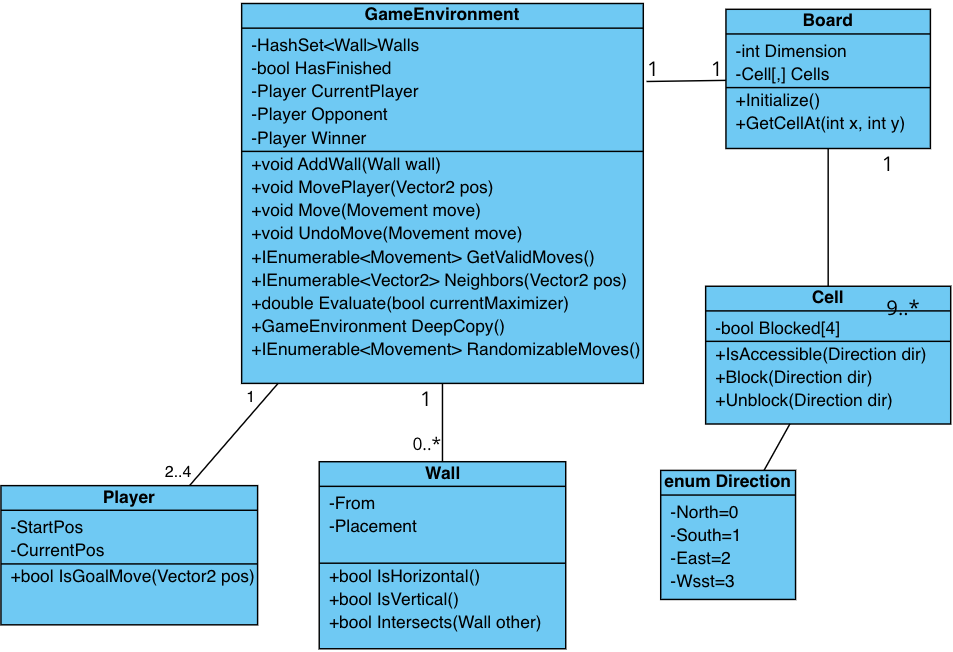
\includegraphics[width=.95\linewidth]{../img/uml_core.png}
    \caption{A UML diagram depicting relationship in the core library}
    \label{fig:core_uml}
\end{figure}

As seen in Figure \ref{fig:core_uml}, the \texttt{GameEnvironment} class implements all interfaces necessary for \gls{AI} integration.

In contrast to the \textbf{Tic-Tac-Toe} implementation we saw earlier in Section \ref{TicTacToe} where \texttt{int} type was used for the \texttt{TMove} parameter, we use a reference type \texttt{Movement} for the \texttt{TMove} parameter, since we need to consider wall placement and player movement, which is difficult to encode and decode as integral values.

\begin{lstlisting}
public abstract class Movement{}

public class Vector2 : Movement{...}

public class Wall : Movement{...};
\end{lstlisting}

This approach makes it easier to identify movement types and therefore easily perform Move/Unmove operations on the game and much more.

We will now describe the core elements of the interfaces that we integrated for this game.

\begin{lstlisting}
public IEnumerable<Movement> GetValidMoves() {
    List<Vector2> neighborMoves;
    //Populate the moves based on whether the neighboring
    //cells are accessible from the cell the current player
    //is in

    List<Wall> possibleWalls;
    //Populate the available wall list. We don't include
    //already placed walls/walls intersecting with already
    //placed walls

    return neighborMoves.Concat(possibleWalls);
}
\end{lstlisting}

Also, as described earlier, for the move and unmove operations, we do not need to decipher the movement by a pre-defined rule like we did in Section \ref{TicTacToe}. We can easily check the underlying type of the abstract Movement type and do operations accordingly.

\begin{lstlisting}
public void Move(Movement move) {
    if (move is Vector2 v2) {
        MovePlayer(v2);
    }
    if (move is Wall wall) {
        AddWall(wall);
    }
    //change turn
}
\end{lstlisting}



\subsection{Project Structure}

The solution consists of six fundamental projects, each written in \gls{Csharp}.

\begin{itemize}
    \item \textbf{Quoridor.Core}\\
        This library project contains the core game logic for Quoridor, and implements all interfaces to allow \gls{AI} algorithms to run.
        
    \item \textbf{Quoridor.AI}\\
        This library project includes all the fundamental interfaces and a generic \gls{AI} algorithms implemented using these interfaces.

    \item \textbf{Quoridor.Common}\\
        This library project includes all common helpers, such as XML parser helper, logging helper, etc.

    \item \textbf{Quoridor.Tests}\\
        This NUnit test project includes all unit tests for robust development.

    \item \textbf{Quoridor.ConsoleApp}\\
        A CLI tool that runs simulations and allows user to play against an opponent with a visual interface.

    \item \textbf{Quoridor.DesktopApp}\\
        A WinForms application that allows user to play against one another or against various \gls{AI}.
\end{itemize}

These projects are inter-connected by references. For example from Figure \ref{fig:proj_dep}, \textbf{Quoridor.AI} is a standalone library that contains all the interfaces, which is referenced by all other projects.
All project dependency structures are depicted in Figure \ref{fig:proj_dep}.

\begin{figure}[!ht]
    \centering
    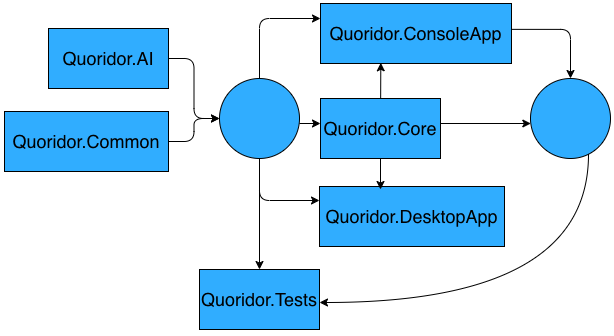
\includegraphics[width=.95\linewidth]{../img/project_structure.png}
    \caption{Quoridor project dependency diagram}
    \label{fig:proj_dep}
\end{figure}
\chapter{Experiments} \label{Experiments}

In this chapter, we define our experiment, the parameters involved in it for different agents and implementations and the final results of the simulation based on the implementation. The main focus of this chapter will be to characterize the complexity for different implementations mainly in terms of average time per move with different implementations and the result of tournament considered between the different agents. The main reason for the experiment is to validate our implementation and to compare the implemented agents including the random and semi-random agent baselines.

\section{Usage}

We use the console application to run all our experiments.

As an example, we provide the following arguments to the console application to simulate 100 games between Parallel-Minimax with a depth of 1 and Semi-Random agents on a game board of dimension 5x5:

\begin{lstlisting}[language=bash]
$dotnet run play -s1=parallelminimaxab -s2=semirandom -dimension=5 -depth=1 -sim -numsim=100
\end{lstlisting}

The aforementioned command produces the following output:

\begin{lstlisting}
===Results===
Player A : Parallel MinimaxAlgorithmABPruning won 99/100 games. Win rate : 99%. Average move time(ms) : 3.04
Player B : Semi-Random won 1/100 games. Win rate : 1%. Average move time(ms) : 1.05
Toal moves made across 100 games : 1781
Average total moves per game : 17
\end{lstlisting}

From the result above, we see that Parallel Minimax took \textbf{1781} moves across 100 games, with an average time of \textbf{3.04 ms} per move, and with an average win rate of \textbf{99\%}.

Documentation for more sample commands for the console application can be found in Appendix \ref{app:consoleapp}.
Also, the scripts used for multiple agent simulations can be found in Appendix \ref{app:scripts}.
 
In this thesis, the average time per move complexity can be defined as the average time taken by the agent to go through each move. The average is performed with respect to the total number of moves made by a particular agent in a game.

\section{Experiment 1 : Minimax depth tuning}

We first consider the implementation of the Minimax algorithm with the depth limited version, alpha-beta pruning version and the parallel version for different Quoridor board dimensions and demonstrate the time complexity of the implemented agents in terms of average time per move. 

For the following experiment, we run all of the 3 implemented variants of the Minimax algorithm including the alpha-beta and the parallel variant, we use the \textbf{Quoridor.ConsoleApp} console application, and simulate 100 games with different board and agent configurations against the semi-random strategy - a total of 36 times (3 variants of minimax x 3 depth x 4 dimensions).

\begin{figure}[!ht]
]
    \centering
    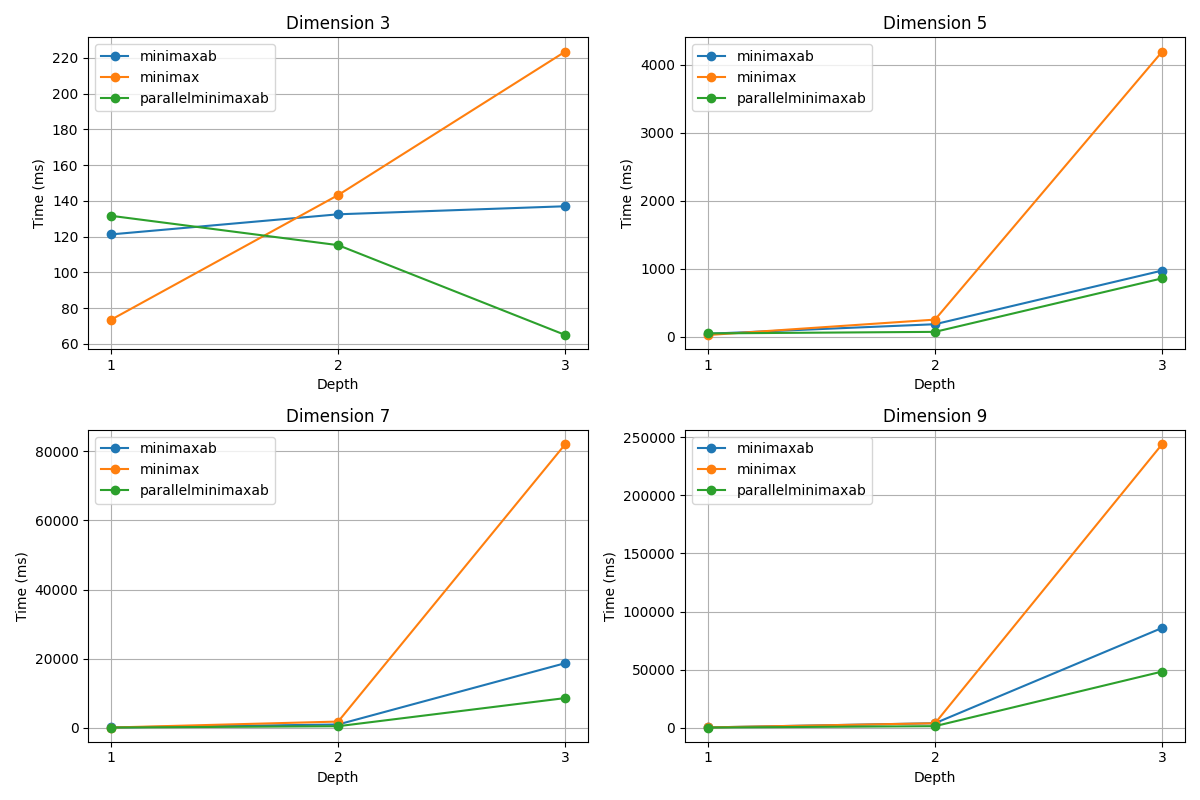
\includegraphics[width=\linewidth]{../img/performance.png}
    \caption{Average move time comparison between all 3 Minimax variants for different board sizes}
    \label{fig:minimax_performance_comp}
\end{figure}

In Figure \ref{fig:minimax_performance_comp}, we can see the average time per move of the Minimax algorithm along with its optimized variants on different board dimensions. In the figure, the dimension refers to the board dimension. For e.g., dimension 3 refers to a board size of 3x3 and so on. Considering the board of large dimension (e.g., 7 and 9), without further optimization, the complexity of implementing the Minimax algorithm for Quoridor is prohibitively high. For example, for depth 3, the move time complexity for the board with dimension 7 is 82 seconds and that for dimension 9 is 244 seconds.

From the figure, it can be inferred that for depth 1, the minimax algorithm without any further optimizations including alpha-beta or parallel implementation performs the fastest. The reason for this is straightforward, as for depth 1, the algorithm only evaluates one further move. In such case, there is not further improvement with alpha beta as we anyways need to evaluate all the nodes. The additional condition checking for the alpha beta implementation for this depth increases the average time per move without any gains. Similarly, the complexity of implementing the parallel algorithm outweighs the simple sequential evaluation hence increasing the time complexity per move without any impact on the performance.

However, for depths more than 1, it can be seen that the time complexity for each move considering alpha-beta pruning and further parallel implementation of the algorithm significantly improves as we increase the considered depth. Below, we have a table showing the improvement of the time complexity considering the minimax algorithm without any further optimization as the baseline.

\begin{table}[!ht]
    \centering
     \begin{tabular}{|c|c|c|c|}\hline
          & Depth 1 & Depth 2 & Depth 3\\ \hline 
          \textbf{Dimension: 3x3}  &    &    &     \\ \hline
          Minimax  &  1  &   1 &   1  \\ \hline
          Minimax alpha-beta &  1.8 &  0.92 &  0.61 \\ \hline
          Minimax alpha-beta parallel & 1.79 & 0.8& 0.29  \\ \hline
          \textbf{Dimension: 5x5}  &    &    &     \\ \hline
          Minimax  &  1  &   1 &   1  \\ \hline
          Minimax alpha-beta &  1.82 &  0.72 &  0.23 \\ \hline
          Minimax alpha-beta parallel & 2.06 & 0.27 & 0.20  \\ \hline
          \textbf{Dimension: 7x7}  &    &    &     \\ \hline
          Minimax  &  1  &   1 &   1  \\ \hline
          Minimax alpha-beta &  1.29 &  0.53 &  0.22 \\ \hline
          Minimax alpha-beta parallel & 1.05 & 0.25 & 0.10 \\ \hline
          \textbf{Dimension: 9x9} &    &    &     \\ \hline
          Minimax  &  1  &   1 &   1  \\ \hline
          Minimax alpha-beta &  1.06 &  1 &  0.35 \\ \hline
          Minimax alpha-beta parallel & 0.43 & 0.33 & 0.19  \\ \hline
     \end{tabular}
     \caption{Relative move-time complexity compared to the baseline minimax algorithm}
     \label{tab:complexity}
 \end{table}

In Table \ref{tab:complexity}, we present the relative move time complexity of the different algorithms with reference to the minimax algorithm for the same depth. Here, we can see that, especially for depth 2 and depth 3, the minimax algorithm, when using the alpha beta pruning and further parallel implementation takes significantly less time. This is especially relevant when considering the large dimension of the Quoridor board as the move time complexity is significantly high. Here, optimization is required for running the algorithm in relatively manageable time.

So, in the experiments that follow, we will use the Parallel Minimax algorithm.

\section{Experiment 2 : 3x3 board}

In this section, we perform various simulations to find out the best parameters for the \gls{MCTS} algorithm, and use those to run head-to-head simulations between all agents to find out the best performing one for the 3x3 game board.

\subsection{MCTS parameter tuning}

The main aim of this experiment is to tune the parameters in the MCTS algorithm, namely the number of iterations and the exploration parameter. Given a relatively small size of the board, each move has a significant impact on the result, where a single miscalculation can lead to an immediate loss. For example, Figure \ref{fig:3x3InitialGameState} depicts the initial game state for the 3x3 configuration. Player A makes a move \texttt{b2} resulting in the game state depicted by Figure \ref{fig:3x3b2movebyA}. Player B now can immediately win with the move \texttt{a2} (it jumps over player A). Considering this, we choose a large number of game iterations, \textbf{500} for MCTS. Higher iteration count allows for a comprehensive evaluation of the game states, accounting for the strategic depth required in the tight confines of a 3x3 board where tactical blunders are less forgivable and can lead to a loss, allowing the algorithm to recognize and avoid simplistic heuristics that may overlook such critical missteps as depicted in figure \ref{fig:3x3BadMove}

\begin{figure}[!ht]
    \begin{subfigure}{0.3\textwidth}
      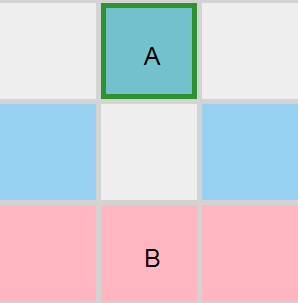
\includegraphics[width=\textwidth]{../img/GameBoard/3_3_board_start.png}
      \caption{Initial game state}
      \label{fig:3x3InitialGameState}
    \end{subfigure}
    \hfill
    \begin{subfigure}{0.3\textwidth}
      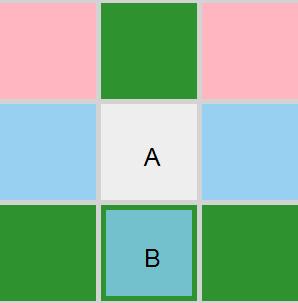
\includegraphics[width=\textwidth]{../img/GameBoard/3_3_mcts_move.png}
      \caption{b2 move by player A}
        \label{fig:3x3b2movebyA}
    \end{subfigure}
    \caption{First bad move by player A leading to a (possible) loss}
\label{fig:3x3BadMove}
\end{figure}

Using \textbf{500} iterations, we conduct an experiment by playing the MCTS agents against two different opponents, A* and Minimax with varying exploration parameters. In this experiment, we consider the minimax algorithm with depth of 2 and simulate 50 games for each exploration parameter. We vary the exploration parameter from 0.6 to 1.4 with a interval of 0.1. As we see on Figure \ref{fig:3x3MCTSTuningAStar}, MCTS algorithm with an exploration parameter of \textbf{0.6} won \textbf{100\%} of the games against the \textbf{A*} algorithm and an average of \textbf{74\%} against the \textbf{Minimax} algorithm (with a depth of 2).

\begin{figure}[!ht]
    \begin{subfigure}{0.5\textwidth}
      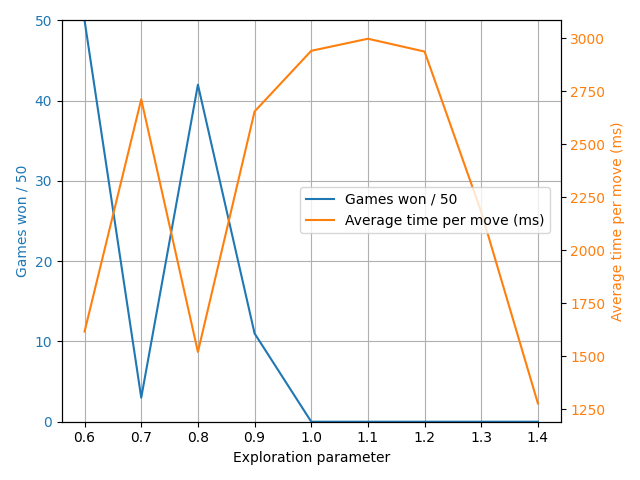
\includegraphics[width=\textwidth]{../img/mcts_exploration_param_grid_search_3_astar.png}
      \caption{MCTS vs A*}
      \label{fig:3x3MCTSTuningAStar}
    \end{subfigure}
    \hfill
    \begin{subfigure}{0.5\textwidth}
      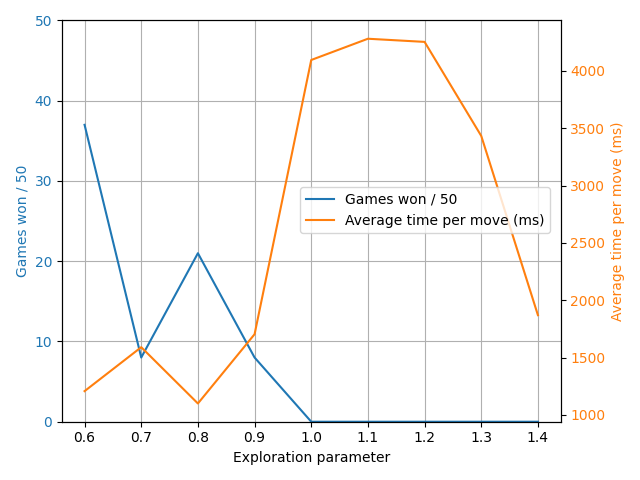
\includegraphics[width=\textwidth]{../img/mcts_exploration_param_grid_search_3_minimax.png}
      \caption{MCTS vs Minimax}
        \label{fig:3x3MCTSTuningMinimax}
    \end{subfigure}
    \caption{Average time per move and win rates of MCTS agent running 500 iterations with varying exploration parameter for board size 3x3}
\label{fig:3x3MCTSTuning}
\end{figure}

Furthermore, as depicted by the graphs in Figure \ref{fig:3x3MCTSTuning}, MCTS algorithm loses all games against the two opponents when the exploration parameter is greater than 1. A parameter greater than 1 excessively prioritizes \textbf{exploration} of states with very few simulations, leading to a neglect on promising strategies already discovered by the MCTS algorithm. This can cause the algorithm to overlook immediate threats or miss direct paths to victory, as evidenced by the total losses incurred at higher parameter values on Figure \ref{fig:3x3MCTSTuning}. In contrast, an exploration parameter less than 1 indicates a balanced approach that weighs the value of \textbf{exploiting} well-performing moves against the potential benefit of exploring new moves. This balance is particularly critical on the small 3x3 board, where each decision carries significant weight. Therefore, an exploration parameter value below 1 is preferred for a 3x3 Quoridor board, as it ensures that the algorithm maintains a focus on exploiting successful strategies while still considering any potential novel moves, leading to more consistent and strategic game play.

\subsection{Results}
In Table \ref{tab:agent_eval_3x3}, we present the tournament result for the agents for the board dimension 3x3 and present the results. For the simulation, we ran the experiment 1000 times between different agents. For the minimax agent, we considered the depth of 2. For \gls{MCTS} agent, we considered the determined optimal exploration parameter of 0.6 and 500 \gls{MCTS} simulations per move.

A value $V_{i,j}$ for agents $i$ and $j$ refers to the average win rate out of 1000 simulations with agent $i$ as player A and agent $j$ as player B.

With these parameters, we can now compare various agents on a board of dimension 3x3.

\begin{table}[!ht]
    \centering
     \begin{tabular}{|c|c|c|c|c|c|}\hline
    \backslashbox{p1}{p2}            & Random & Semi-Random & A*  & Minimax & MCTS \\ \hline 
    Random      &        &    31.3     & 6.6 &   5.3   &  0   \\ \hline
    Semi-Random &   73.5 &             & 11.5&   10.2  &  0  \\ \hline
    A*          &   92.2 &    90.2     &     &   0     &  0   \\ \hline
    Minimax     &   92.4 &    88.9     & 8.2 &         &  0   \\ \hline
    MCTS        &   90   &    74.3     &  100 &   74    &      \\ \hline
     \end{tabular}
     \caption{Agent comparison for dimension 3x3. The values in the
table represent the total win percentage of the agent in the row of the table when competing against the agent in the column of the table.}
     \label{tab:agent_eval_3x3}
 \end{table}

\section{Experiment 3 : 5x5 board}

Following the results of the 3x3 board experiment as presented in Table \ref{tab:agent_eval_3x3}, we would also like to find out the ideal \gls{MCTS} parameters for the 5x5 variant and run a head-to-head tournament betweeen all our implemented agents.

\subsection{MCTS parameter tuning}

For this experiment, we consider a Quoridor board of size 5x5 and play against a Minimax agent with a depth 2 and like the previous scenario, perform 50 experiments per parameter we are interested in.

First, we perform a grid search to find the ideal number iterations for the 5x5 board, using average win-rate as our deciding factor. We iterate over a range of 30 to 240 with an interval of 30 and run 50 simulations, all while using a theoretical optimal exploration parameter of $\sqrt{2}$ \citep{kocsis2006bandit}.

\begin{figure}[!ht]
    \centering
    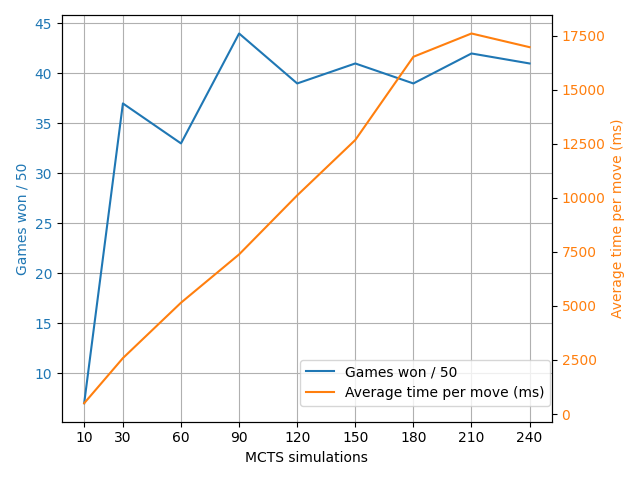
\includegraphics[width=0.7\linewidth]{../img/mcts_simulation_grid_search.png}
    \caption{Average time per move and win rates of MCTS agent with varying simulations for board size 5x5}
    \label{fig:mcts_simulations}
\end{figure}

In Figure \ref{fig:mcts_simulations}, we see that after 90 simulations, the additional marginal number of game won does not increase, although the time per move increases. Hence, optimizing the number of simulations can be important to limiting the complexity of the \gls{MCTS} agent.

\begin{figure}[!ht]
    \centering
    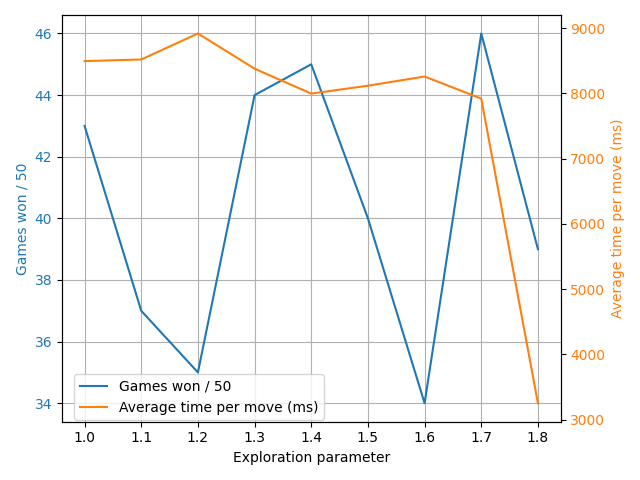
\includegraphics[width=0.7\linewidth]{../img/mcts_exploration_param_grid_search.png}
    \caption{Average time per move and win rates of MCTS agent with varying exploration parameter for board size 5x5}
    \label{fig:mcts_exp_simulations}
\end{figure}

Likewise, in Figure \ref{fig:mcts_exp_simulations}, we use 90 iterations we deduced from Figure \ref{fig:mcts_simulations} to find the optimal exploration parameter based on the number of games won varied with different exploration parameters. From Figure \ref{fig:mcts_exp_simulations}, we see that with an optimal exploration parameter of \textbf{1.7}, the win rate for the agent is high i.e 46 wins out of 50 games.

\subsection{Results}
 
 Firstly, we can observe that the Random agent, as expected, does poorly against all other agents. However, in the 3x3 board, the Random agent still wins a third of the time again Semi-Random agent and a few times against the even the A-star and the Minimax agents. From the table, it can also be observed that the \gls{MCTS} agent performs the best in the 3x3 board as it almost does not lose any games against the any other agents.

\begin{table}[!ht]
    \centering
     \begin{tabular}{|c|c|c|c|c|c|}\hline
     \backslashbox{p1}{p2} & Random & Semi-Random & A*  & Minimax & MCTS \\ \hline 
    Random      &        &    5.8      &  0  &   0     &   0  \\ \hline
    Semi-Random &   93.6 &             & 0.3 &   1.9   &  3.3 \\ \hline
    A*          &   100  &    99.7     &     &   22.7     & 73.3 \\ \hline
    Minimax     &   99.9 &    99.4     & 87.3 &         & 33.3 \\ \hline
    MCTS        &   100  &    100      & 56.7&   92    &      \\ \hline
     \end{tabular}
     \caption{Agent comparison for dimension 5x5. The values in the
table represent the total win percentage of the agent in the row of the table when competing against the agent in the column of the table.}
     \label{tab:agent_eval_5x5}
 \end{table}

 In Table \ref{tab:agent_eval_5x5}, we present the result of the tournament when considering a Quoridor board of dimension 5. For this board dimension, we again consider the total number of simulation runs as 1000. For the minimax agent, we considered the depth as 2. For the \gls{MCTS} simulation, we considered the determined optimal exploration parameter of 1.7 and ran 90 simulations per move.
 
 From the table, we can observe that considering a board of a larger dimension, both the Random and the Semi-Random agents perform poorly since they require a large number of good moves in a sequence to win, which is less-likely to happen. From the table, we can also see that the \gls{MCTS} algorithm performs best against all the algorithms, winning more than 90\% of its games except for the A-star agent where it wins more than half of its games. Another surprising factor is that the A-star algorithm which only considers the distance from the start position and end position as the main cost functions performs much better than the minimax algorithm.  

\section{Experiment 4: 7x7 board}

For the \gls{MCTS} agent, since the average move time was 34.4 seconds with the available simulation hardware, we could only perform 100 simulations. Additionally, the simulation run time also prevented us from using an optimized parameter. Hence, we used the theoretical optimal parameter of $\sqrt{2}$ \citep{kocsis2006bandit} for this dimension. For the minimax agent, we considered the implementation with depth 2. 

\begin{table}[!ht]
    \centering
     \begin{tabular}{|c|c|c|c|c|c|}\hline
\backslashbox{p1}{p2}& Random & Semi-Random & A*  & Minimax & MCTS \\ \hline 
    Random      &        &    0.2        &  0  &   0     &  0    \\ \hline
    Semi-Random &   99.6 &             & 0.2 &  0.7    &  0.2 \\ \hline
    A*          &   100  &    99.7     &     &   18.2     &  2    \\ \hline
    Minimax     &   100  &    99.3     & 79.8 &         & 58 \\ \hline
    MCTS        &    100    & 100  &  3   &        44 &      \\ \hline
     \end{tabular}
     \caption{Agent comparison for dimension 7x7. The values in the
table represent the total win percentage of the agent in the row of the table when competing against the agent in the column of the table.}
     \label{tab:agent_eval_7x7}
 \end{table}
 
In Table \ref{tab:agent_eval_7x7}, we illustrate the result of the tournament when considering a board of dimension 7x7. For this dimension we also ran 1000 simulations for all the agents except for the \gls{MCTS} agent. 

Here, the performance of the random agent is significantly worse compared to the previous boards as it fails to win any games against A-star, minimax and MCTS agents. Unlike the previous smaller boards, in this instance, the minimax algorithm performs much better against A-star algorithm as it wins almost all of its games. From this, we can conclude that the strategical play with the minimax algorithm for larger board is much more significant than the simple cost function oriented traversal strategy of the A-star algorithm.
 
From the above tournament simulation presented in Table \ref{tab:agent_eval_7x7}, we can conclude that the board dimension does have an effect on the strategy that might be used. For board of smaller dimensions such as 3 and 5, simpler strategies such as  random and semi-random in some cases can be enough to get some wins against more strategical agents such as the minimax agent. However, as the board dimension gets higher, the required strategy is very prominently visible as semi-random and random agents win almost no games against the other agents.
\chapter*{Conclusion}
\addcontentsline{toc}{chapter}{Conclusion}


%%% Bibliography
%%% Bibliography (literature used as a source)
%%%
%%% We employ bibTeX to construct the bibliography. It processes
%%% citations in the text (e.g., the \cite{...} macro) and looks up
%%% relevant entries in the bibliography.bib file.
%%%
%%% The \bibliographystyle command selects, which style will be used
%%% for references from the text. The argument in curly brackets is
%%% the name of the corresponding style file (*.bst). Both styles
%%% mentioned in this template are included in LaTeX distributions.

\bibliographystyle{plainnat}    %% Author (year)
% \bibliographystyle{unsrt}     %% [number]

\renewcommand{\bibname}{Bibliography}

%%% Generate the bibliography. Beware that if you cited no works,
%%% the empty list will be omitted completely.

\bibliography{bibliography}

%%% If case you prefer to write the bibliography manually (without bibTeX),
%%% you can use the following. Please follow the ISO 690 standard and
%%% citation conventions of your field of research.

% \begin{thebibliography}{99}
%
% \bibitem{lamport94}
%   {\sc Lamport,} Leslie.
%   \emph{\LaTeX: A Document Preparation System}.
%   2nd edition.
%   Massachusetts: Addison Wesley, 1994.
%   ISBN 0-201-52983-1.
%
% \end{thebibliography}


%%% Figures used in the thesis (consider if this is needed)
%\listoffigures

%%% Tables used in the thesis (consider if this is needed)
%%% In mathematical theses, it could be better to move the list of tables to the beginning of the thesis.
%\listoftables

%%% Abbreviations used in the thesis, if any, including their explanation
%%% In mathematical theses, it could be better to move the list of abbreviations to the beginning of the thesis.
\printglossaries


%%% Attachments to the bachelor thesis, if any. Each attachment must be
%%% referred to at least once from the text of the thesis. Attachments
%%% are numbered.
%%%
%%% The printed version should preferably contain attachments, which can be
%%% read (additional tables and charts, supplementary text, examples of
%%% program output, etc.). The electronic version is more suited for attachments
%%% which will likely be used in an electronic form rather than read (program
%%% source code, data files, interactive charts, etc.). Electronic attachments
%%% should be uploaded to SIS and optionally also included in the thesis on a~CD/DVD.
%%% Allowed file formats are specified in provision of the rector no. 72/2017.
\appendix
\chapter{Attachments}

\section{First Attachment}
\label{app:repository}
The link to the implementation can be found here: 
\url{https://github.com/devyanshuk/Quoridor}


\section{Second Attachment}
\label{app:consoleapp}
The link to the Console App user documentation can be found here: \url{https://github.com/devyanshuk/Quoridor/blob/main/Quoridor/Quoridor.ConsoleApp/README.md}

\section{Third Attachment}
\label{app:desktopapp}
The link to the Desktop App user documentation can be found here: \url{https://github.com/devyanshuk/Quoridor/blob/main/Quoridor/Quoridor.DesktopApp/README.md}

\section{Fourth Attachment}
\label{app:programmerdoc}
The link to the Programmer's documentation can be found here:
\url{https://github.com/devyanshuk/Quoridor/blob/main/Quoridor/Thesis/ProgrammerDoc.md}


\openright
\end{document}
